\documentclass{article}
% Package to manage page layout
\usepackage[margin=2cm, includefoot, footskip=30pt]{geometry}

\setlength\parindent{0pt}
\setlength{\parskip}{1em}

%%%%%%%PACKAGES HERE%%%%%%%
\usepackage{amsmath}
\usepackage{amsthm}
\usepackage{amssymb}
\usepackage{hyperref}
\usepackage{standalone}
\usepackage{subcaption}
\usepackage{adjustbox}
\usepackage{tikz}
\usepackage{booktabs}
\usepackage{multicol,multirow,array}
\usepackage{graphicx}
\usepackage{algorithm,algorithmic}
\usepackage{authblk}
\usepackage{tabularx}
\usepackage{color, colortbl}
\usetikzlibrary{er,positioning, calc, patterns}
\usetikzlibrary{decorations.pathreplacing}

\definecolor{Gray}{gray}{0.92}
\definecolor{background}{RGB}{5, 66, 81}

\setcounter{secnumdepth}{4}
\setcounter{tocdepth}{4}

\theoremstyle{definition}
\newtheorem{definition}{Definition}[section]

%%%%%%%%%%%%%%%%%%%%%%%%%%%%%%%PARAMETERS%%%%%%%%%%%%%%%%%%%%%%%%%%%%%%%%%%%%%%%
\newcommand{\totalarticles}{\input{assets/total_articles.txt}}
\newcommand{\manual}{\input{assets/prov_manual.txt}}
\newcommand{\authors}{\input{assets/number_of_authors.txt}}
\newcommand{\edges}{\input{assets/num_Edges.txt}}
\newcommand{\isolated}{\input{assets/num_Isolated_nodes.txt}}
\newcommand{\isolatedpercentage}{\input{assets/perce_Isolated_nodes.txt}}
\newcommand{\connectedcomponents}{\input{assets/num_Connected_components.txt}}
\newcommand{\communities}{\input{assets/num_Communities.txt}}
\newcommand{\largestcc}{\input{assets/Size_of_largest_component.txt}}
\newcommand{\clustering}{\input{assets/Clustering_coeff.txt}}
%%%%%%%%%%%%%%%%%%%%%%%%%%%%%%%%%%%%%%%%%%%%%%%%%%%%%%%%%%%%%%%%%%%%%%%%%%%%%%%%
%%%%%%%%%%%%%%%%%%%%%%%%%%%%%%%%%%%%%%%%%%%%%%%%%%%%%%%%%%%%%%%%%%%%%%%%%%%%%%%%
\title{A bibliometric study of collaboration and influence in the field of
the Iterated Prisoner's Dilemma}

\author[1]{Nikoleta E. Glynatsi}
\author[1]{Vincent A. Knight}

\affil[1]{Cardiff University, School of Mathematics, Cardiff, United Kingdom}
\date{}
\setcounter{Maxaffil}{0}
\renewcommand\Affilfont{\itshape\small}
\begin{document}

\maketitle

\begin{abstract}
This manuscript explores the collaborative behaviour of authors in the field
of the Prisoner's Dilemma using bibliometric analysis, topic modeling, and
the co-authorship network. The results demonstrate that the Prisoner's
Dilemma is a field of continued interest and  a collaborative field. Authors
are very like to cooperate with a collaborator's co-author and single author
publications are rare. The co-authorship network however suggests that
authors do not influence or gain much information by their connections,
unless they are connected to a ``main'' group of authors. The articles
collected for this work are classified based on the language of their
abstracts in five different topics, and the results are additionally verified by
the topics' networks.
\end{abstract}

\section{Introduction}\label{section:introduction}

The Prisoner's Dilemma (PD) is a well known game used since its introduction in the
1950's~\cite{Flood1958} as a framework for studying the emergence of
cooperation; a topic of continuing interest for mathematical,
social~\cite{Perc2008}, biological~\cite{Turner1999} and
ecological~\cite{Wu2011} sciences. This manuscript presents a bibliometric
analysis of the Prisoner's Dilemma field, in the interest of understanding the
number of publications over the years, the research trends within the
field, and mainly to assess the collaborative behaviour
of the authors in the field of cooperation itself.

As discussed in~\cite{youngblood2018}, bibliometrics (the statistical analysis
of published works originally described by~\cite{pritchard1969}) has been used
to support historical assumptions about the development of fields
\cite{raina1998}, identify connections between scientific growth and policy
changes \cite{das2016}, develop a quantitative understanding of author
order~\cite{sekara2018}, and investigate the collaborative structure of an
interdisciplinary field~\cite{Liu2015}. Most academic research is undertaken in
the form of collaborative effort and as~\cite{Kyvik2017} points out, it is
rational that two or more people have the potential to do better as a group
than individually. Collaboration in groups has a long tradition in experimental
sciences and it has be proven to be productive according
to~\cite{Etzkowitz1992}. The number of collaborations can be very different
between research fields and understanding how collaborative a field is not
always an easy task. Several studies tend to consider academic citations as a
measure for these things. A blog post published by Nature~\cite{nature_blog}
argues that depending on citations can often be misleading because the true
number of citations can not be known. Citations can be missed due to data entry
errors, academics are influenced by many more papers than they actually cite and
several of the citations are superficial.

A more recent approach to measure collaborative behaviour is to use the
co-authorship network, as described in~\cite{Liu2015}. Using this approach has many
advantages as several graph theoretic measures can be used as proxies to explain
authors relationship. In~\cite{Liu2015}, they analyse the development of the
field ``evolution of cooperation'' using this approach. The topic ``evolution of
cooperation'' is a multidisciplinary field which also includes a large number of
publications on the PD. This paper builds upon the work done by~\cite{Liu2015}
and extends their methodology. Though in \cite{Liu2015}, they considered a data
set from a single source, Web of Science, the data set described here, archived
at~\cite{pd_data_2018}, has been collected from five different sources.
Co-authorship networks have also been used in~\cite{youngblood2018, Li2019}.
In~\cite{youngblood2018} it is used for identifying the subdisciplines the interdisciplinary
field of cultural evolution so that they can describe each subdiscipline and
investigate trends in collaboration and productivity, and in~\cite{Li2019} for examining
the long-term impact of co-authorship with established, highly-cited scientists
on the careers of junior researchers.

The Prisoner's Dilemma, much like cultural evolution and evolution of cooperation,
has attracted the attention of researchers across fields, and more specifically
its iterated version, the Iterated Prisoner's Dilemma (IPD). This is due to
the game not only being mathematically
intriguing~\cite{Press2012} but also being used a model of
social~\cite{Zimmermann2005} and biological~\cite{Doebeli2005} interactions and
having applications in numerous fields such as healthcare~\cite{Turner1999}. The
game was chosen for this work as a result of it being a specific topic with
publications across the academic fields.

The type of analysis  which is carried out in this work has been carried out
before in~\cite{Liu2015} and~\cite{youngblood2018}. The novelty here is to
consider a new data set on a specific game theoretic topic and approaches not considered in
either works, such as topic modeling~\cite{Blei2003} and centrality measures.
The data set of this work contains \totalarticles
articles' metadata on the IPD that have been collected from five different
prominent sources. The methodology used in this manuscript, which includes the
data collection, is covered in Section~\ref{section:methodology}. The results regarding,
the amount of publications and the topics of the field over the years are
described in Section~\ref{section:results}. In
Section~\ref{section:co_authorship}, graph theoretical methods are used to
ascertain the level of collaborative nature of the field and identify influence.

\section{Methodology}\label{section:methodology}

Academic articles are accessible through scholarly databases. Several databases
and collections today offer access through an open application protocol
interface (API). An API allows users to query directly a journal's database and
bypass the graphical user interface. Interacting with an API has two phases:
requesting and receiving. The request phase includes composing a url with the
details of the request. For example,
\url{http://export.arxiv.org/api/query?search_query=abs:prisoner's
dilemma&max_results=1} represents a request message. The first part of the
request is the address of the API. In this example the address corresponds to
the API of arXiv. The second part of the request contains the search arguments.
In this example it is requested that the word `prisoners dilemma' exists within
the article's title. The format of the request message is different from API to
API. The receive phase includes receiving a number of raw metadata of articles
that satisfies the request message. The raw metadata are commonly received in
extensive markup language (xml) or Javascript object notation (json)
formats~\cite{nurseitov2009}. Similarly to the request message, the structure of
the received data differs from journal
to journal.

The data collection is crucial to this study. To ensure that this study can be
reproduced all code used to query the different APIs has been packaged as a
Python library and is available online~\cite{nikoleta_2017}. The software could
be used for any type of projects similar to the one described here,
documentation for it is available at:
\url{http://arcas.readthedocs.io/en/latest/}. Project~\cite{nikoleta_2017} allow
users to collect articles from a list of APIs by specifying just a single
keyword. Articles for which any of the terms

\begin{itemize}
    \item \{``prisoner's dilemma'',
    ``prisoners dilemma'', ``prisoner dilemma'', ``prisoners evolution'', ``prisoner
    game theory''\}
\end{itemize}

existed within the title, the abstract or the text are included
in the analysis. Four prominent journals in the field and a preprint server
were used as sources to collect data for this analysis:

\begin{multicols}{2}
    \begin{itemize}
        \item arXiv~\cite{mckiernan2000}; a repository of electronic preprints.
        It consists of scientific
        papers in the fields of mathematics, physics, astronomy, electrical engineering,
        computer science, quantitative biology, statistics, and quantitative finance,
        which all can be accessed online.
        \item PLOS~\cite{plos}; a library of open access journals and other scientific literature
        under an open content license. It launched its first journal, PLOS Biology,
        in October 2003 and publishes seven journals, as of October 2015.
        \item IEEE Xplore Digital Library (IEEE)~\cite{ieee}; a research database for discovery
        and access to journal articles, conference proceedings, technical standards,
        and related materials on computer science, electrical engineering and electronics,
        and allied fields. It contains material published mainly by the Institute of
        Electrical and Electronics Engineers and other partner publishers. 
        \item Nature~\cite{nature}; a British multidisciplinary scientific journal,
        first published on 4 November 1869. It was ranked the world's most cited
        scientific journal by the Science Edition of the 2010 Journal Citation Reports
        and is ascribed an impact factor of 40.137, making it one of the world's
        top academic journals.
        \item Springer~\cite{springer}; a leading global scientific publisher of
        books and journals. It publishes close to 500 academic and professional
        society journals.
    \end{itemize}
\end{multicols}

The data set is archived and available at~\cite{pd_data_2018}. Note that the latest data
collection was performed on the \(30^{\text{th}}\) November 2018.
% TODO Ensure this stay accurate

The data set contains a total of \totalarticles articles. These will be classified
into research topics using \textbf{topic modeling}, a computational method
designed to summarize large collections of texts by a small number of
conceptually connected topics or themes~\cite{Blei2003, Grimmer2013}. The text
used for each article is its abstract. Topic modeling analyses the patterns
with which words co-occur in the abstracts, and then a topic is defined by a
probability distribution over words. So in one topic the word ``cooperation''
would have a high weighting, and in another topic it would have a low weighting.
Similarly for all the words that have been captured by the abstracts. Note that
the words have been simplified by ignoring order and removing stop words.
Once the topics are defined, as a distribution over words, articles are assigned
to them based on which topic has the highest percentage contribution for a given
article. For example let the words that contribute to Topic A be:
\(0.039 \times\)``cooperation'', \(0.028 \times\)``study'' and \(0.026 \times\)``human''
and for Topic B: \(0.020 \times\)``cooperation'', \(0.028 \times\)``agents'' and
\(0.026 \times\)``strategies''. A document with abstract ``The
study of cooperation in humans'' is assigned to Topic A because \((0.039 + 0.028 + 0.026)
> 0.020\).

A issue regarding the technique is that the
number of topics need to be specified in advance before running the algorithm.
The suitable number of topics presented here are based on the topic coherence
measure~\cite{Roder2015} and on the minimisation of overlapping words within two
topics. Note that the minimisation of overlapping words is done manually
by the authors.

The relationship between the authors within a field will be modeled as a graph
\(G = (V_G, E_G)\) where \(V_G\) is the set of nodes and \(E_G\)  is the set of
edges. The set \(V_G\) represents the authors and an edge connects two authors
if and only if those authors have written together. The co-authorship network is
constructed using the main data set~\cite{pd_data_2018} and the open source package
\cite{networkx}. The PD network is denoted as \(G\) where the
number of unique authors \(|V(G)|\) is \authors and \(|E(G)|\) is \edges.
All authors' names were formatted as their last name and first name (i.e.
Martin A. Nowak to Martin Nowak). This was done to avoid errors such as Martin
A. Nowak and Martin Nowak being treated as a different person. There are some
authors for which only their first initial was found and are left this way.

Collaborativeness will be analysed using measures such as, isolated nodes,
connected components, clustering coefficient, communities, modularity and average degree.
These measures show the number of connections authors can have
and how strongly connected these people are. The number of isolated nodes is the
number of nodes that are not connected to another node, thus the
number of authors that have published alone. The average degree denotes the average
number of neighbours for each nodes, i.e. the average number of collaborations
between the authors.
A connected component is a maximal set of nodes such that each pair of nodes is
connected by a path~\cite{Easley2010}. The number of connected components as well as the size of the
largest connected component in the network are reported.
The size of the largest connected component represents the scale of the central cluster
of the entire network, as will discussed in the analysis section.
Clustering coefficient and modularity are also calculated. The clustering
coefficient, defined as 3 times the number of triangles on the graph divided
by the number of connected triples of nodes, is a local measure of the degree to
which nodes in a graph tend to cluster together
in a clique~\cite{Easley2010}. It is precisely the probability that the collaborators
of an author also write together.
In comparison, modularity is a global measure designed to measure the strength of
division of a network into communities. The number of communities will be reported
using the Clauset-Newman-Moore method~\cite{clauset2004}. Also the modularity index
is calculated using the Louvain method described in~\cite{Blondel2008}. The value
of the modularity index can vary between \([-1, 1]\), a high value of modularity
corresponds to a structure where there are dense connections between the nodes within
communities but sparse connections between nodes in different communities.
That means that there are many sub communities of authors that write together
but not across communities.
Two further points are aimed to be explored in this work, (1) which people control the flow
of information;
as in which people influence the field the most and (2) which are the authors that
gain the most from the influence of the field. To measure these concepts
centrality measures are going to be used.
Centrality measures are often used to understand different
aspects of social networks~\cite{Landherr2010}. Two centrality measures have been
chosen for this paper and these are closeness and betweenness centrality.

\begin{enumerate}
    \item In networks some nodes have a short distance to a lot of nodes and
    consequently are able to spread information on the network very effectively.
    A representative of this idea is \textbf{closeness centrality}, where a node
    is seen as centrally involved in the network if it requires only few
    intermediaries to contact others and thus is structurally relatively
    independent. Here, this is interpreted as a influence. Authors with a high
    value of closeness centrality, are the authors that spread scientific
    knowledge easier on the network and they have high influence.
    \item Another centrality measure is the \textbf{betweenness centrality},
    where the determination of an author's centrality is based on the quotient
    of the number of all shortest paths between nodes in the network that
    include the node in question and the number of all shortest paths in the
    network. In betweenness centrality the position of the node matters. Nodes
    with a higher value of betweenness centrality are located in positions that
    a lot of information pass through, this is interpreted as the gain from
    the influence, thus these authors gain the most from their networks.
\end{enumerate}

In the next sections the methodology discussed here is applied to the data
set and results regarding the publications and collaborativeness of the field
are presented.

\section{Initial Analysis}\label{section:results}

The data set~\cite{pd_data_2018} consists of \totalarticles articles with
unique titles. In case of duplicates the preprint version of an article
(collected from arXiv) was dropped. Of these \totalarticles articles, \manual
have not been collected from the aforementioned APIs but have been manually
added because they are of interest to the authors. A similar approach was
used in~\cite{Liu2015} where a number of articles were manually
added to the data set. A more detailed summary of the articles' provenance is
given by Table~\ref{table:provenance}. Only 3\% of the data set consists of
articles that were manually added and 27\% of the articles were collected from
arXiv.

\begin{table}[!hbtp]
    \begin{center}
    \resizebox{.4\textwidth}{!}{
    \begin{tabular}{lrr}
\toprule
{} &  \# of Articles &  Percentage \\
provenance &                &             \\
\midrule
Manual     &             89 &        2.92 \\
IEEE       &            295 &        9.67 \\
Springer   &            458 &       15.01 \\
PLOS       &            482 &       15.79 \\
Nature     &            673 &       22.05 \\
arXiv      &           1055 &       34.57 \\
\bottomrule
\end{tabular}
}
    \end{center}
    \caption{Articles' provenance for the main data set~\cite{pd_data_2018}.}
    \label{table:provenance}
\end{table}

The average number of publications per year is denoted as \(\mu_P =
\frac{N_A}{N_Y}\) where \(N_A\) is the total number of articles and \(N_Y\) is
the years of publication. The years of publication is calculated as the range
between the collection date and the first published article, for each
provenance, within the data. These averages are summarised in
Table~\ref{table:publication_rates}. Overall an average of 43 articles are
published per year on the topic. The most significant contribution to this
appears to be from arXiv with 11 articles per year, followed by Springer with 9
and PLOS with 8.
Though the average publication offers insights about the publications of the
fields, it remains a constant number. The data handled here is a time
series starting in 1950s, when the game was introduced, until 2018 (Figure~\ref{fig:timeseries}). 
Two observations can be made from Figure~\ref{fig:timeseries}.

\begin{table}[!hbtp]
    \begin{center}
    \resizebox{.15\textwidth}{!}{
    \begin{tabular}{lr}
\toprule
{} &  Av. Yearly publication \\
\midrule
IEEE     &                     5.0 \\
PLOS     &                     8.0 \\
Springer &                     9.0 \\
Nature   &                    11.0 \\
arXiv    &                    16.0 \\
Overall  &                    49.0 \\
\bottomrule
\end{tabular}
}
    \end{center}
    \caption{Average yearly publication $(\mu_P)$ for main data set~\cite{pd_data_2018}.}
    \label{table:publication_rates}
\end{table}

\begin{enumerate}
    \item There is a steady increase to the number of publications since the
    1980s and the introduction of computer tournaments~\cite{Axelrod1981}.
    \item There is a decrease in 2017-2018. This is due to our data set being
    incomplete. Articles that have been written in 2017-2018 have either not
    being published or were not retrievable by the APIs at the time of writing
    this manuscript.
\end{enumerate}

These observations can be confirmed by studying the time series.
Using~\cite{scipy}, an exponential distribution is fitted to the data from
1980-2016 (Figure~\ref{fig:fitting}).
The fitted model can be used to forecast the behaviour of the field for the
next 5 years. The forecasted periods are plotted in
Figure~\ref{fig:forecasting}. The time series has indicated a slight decrease
however the model forecasts that the number of publications will keep
increasing, thus demonstrating that the field of the IPD
continues to attract academic attention.

\begin{figure}[!hbtp]
\begin{minipage}{.45\textwidth}
    \centering
    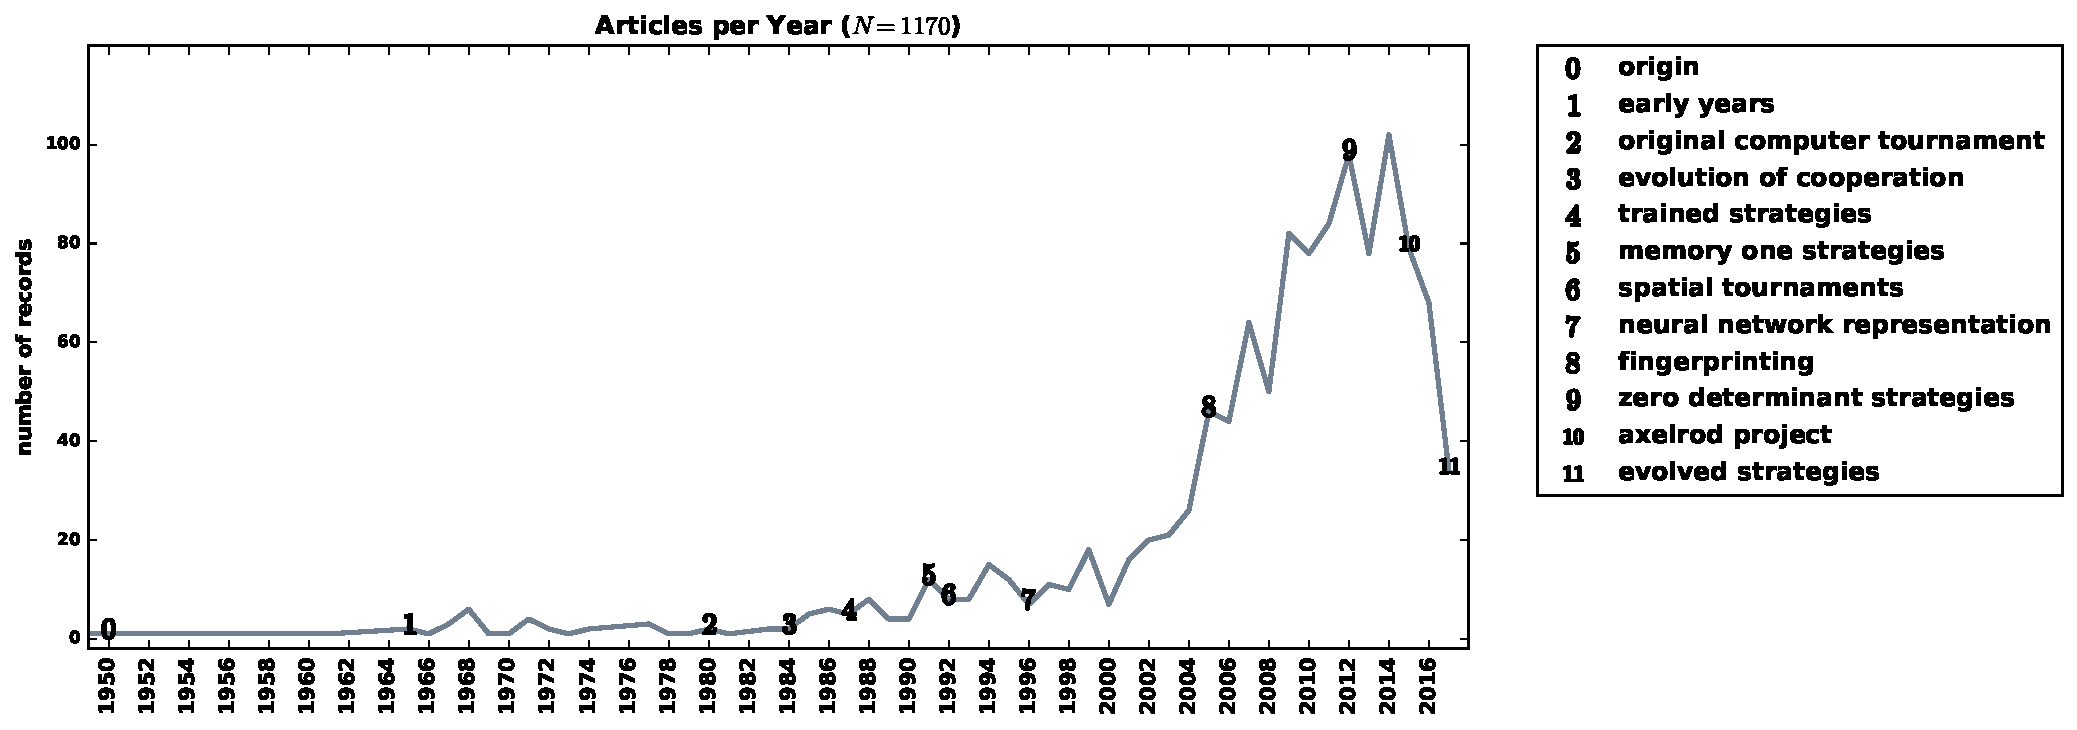
\includegraphics[width=.9\textwidth]{./assets/images/timeline.pdf}
    \caption{Line plot; number of articles published on the PD 1950-2019.}\label{fig:timeseries}
\end{minipage}
\begin{minipage}{.45\textwidth}
    \centering
    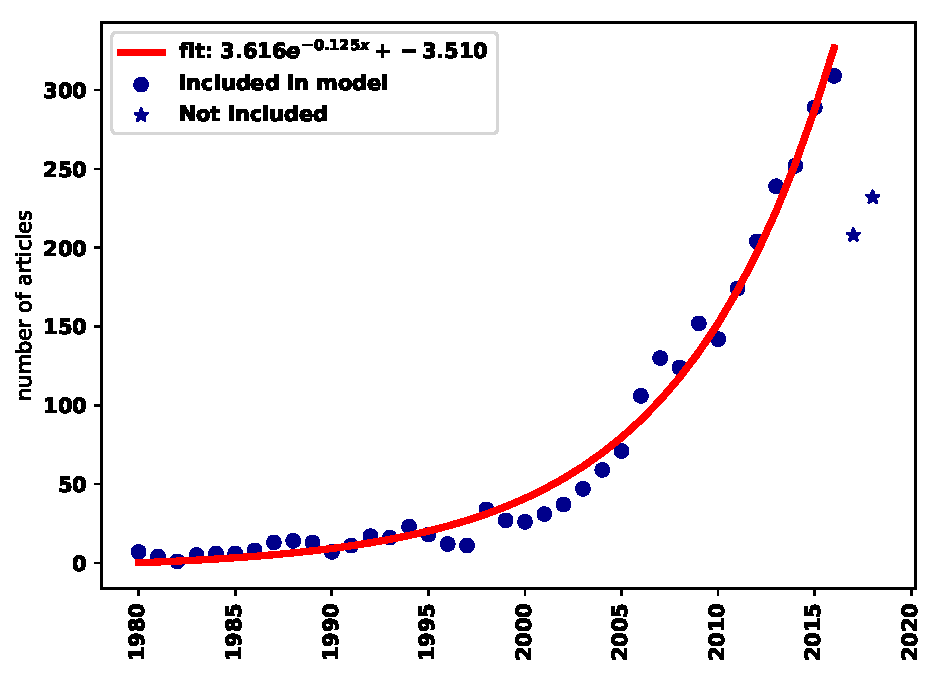
\includegraphics[width=.9\textwidth]{./assets/images/fitting.pdf}
    \caption{Scatter plot; number of articles published on the PD 1980-2019.}\label{fig:fitting}
\end{minipage}
\end{figure}

\begin{figure}[!hbtp]
    \centering
    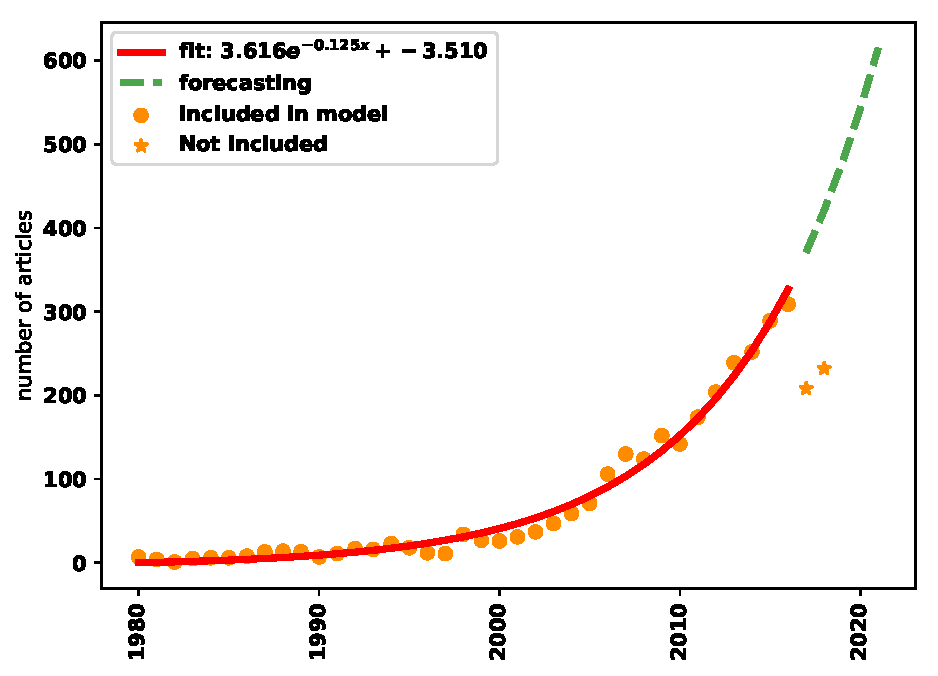
\includegraphics[width=.45\textwidth]{./assets/images/forecasting.pdf}
    \caption{Forecast for 2017-2022.}\label{fig:forecasting}
\end{figure}

The overall collaboration index (CI) or the average number of authors on
multi-authored papers is 3.2. Thus on average a non single author publication in
the PD has 3 authors. The interdisciplinary field of cultural evolution was also
reported to have a CI of 3~\cite{youngblood2018} and from a blog post published
in Nature~\cite{nature_author_blog} it can be seen that other fields such as
Astronomy and Astrophysics, Genetics and Heredity, Nuclear and Particle Physics
have most likely 3 authors. The CI index over time is also given in
Figure~\ref{fig:ci_over_time}. There are some peaks in the early years 1969 and
1980, however, a steady increase appears to happen after 2004. This could
be an effect of better communication tools being introduced around that time
which enabled more collaborations between researchers. The collaborative
behaviour will be explored in more details in the following section using the
co-authorship network.

\begin{figure}[!hbtp]
    \centering
    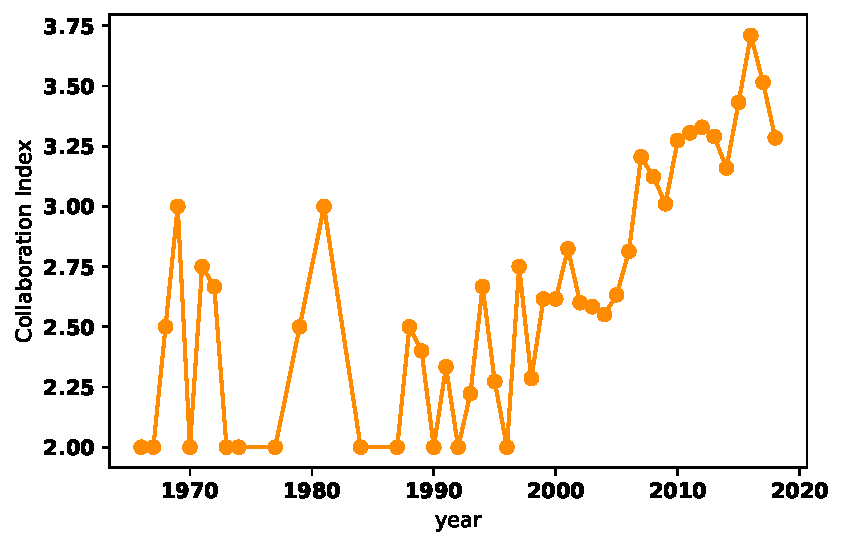
\includegraphics[width=.5\textwidth]{./assets/images/collaborative_index.pdf}
    \caption{Collaboration index over time.}\label{fig:ci_over_time}
\end{figure}

There are a total of \authors unique authors in~\cite{pd_data_2018} and several of them
have had multiple publications collected. The highest number of articles
collected for an author is 83 publications for Matjaz Perc. The logged
distribution of number of papers per author is given by
Figure~\ref{fig:num_papers_per_author} and it can be seen that Matjaz Perc is an
outlier. Mainly the authors have had 1 to 6 publications gathered by the data
collection.

\begin{figure}[!hbtp]
    \centering
    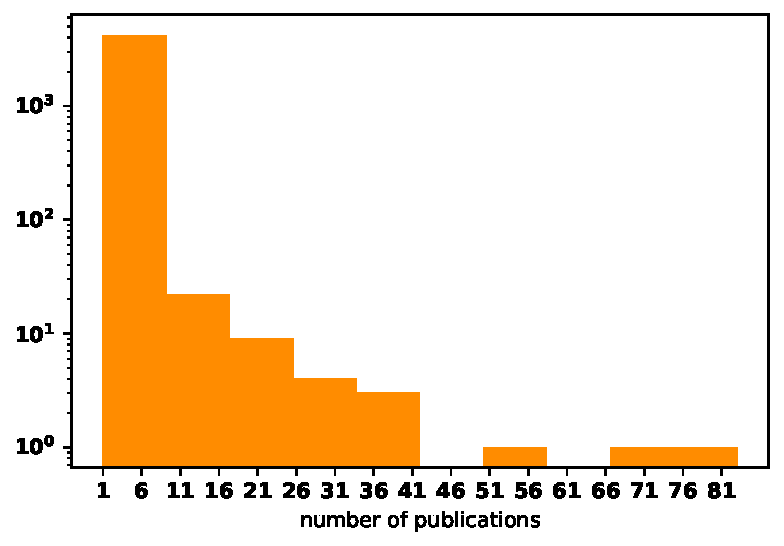
\includegraphics[width=.5\textwidth]{./assets/images/papers_per_author.pdf}
    \caption{Logged distribution of number of papers per author.}
    \label{fig:num_papers_per_author}
\end{figure}

Topic modeling has been applied to the data set using~\cite{rehurek_lrec} and
the \totalarticles articles have been classified into 5 different topics. The
number of total topics was chosen based on the coherence value and the
minimisation of overlapping words within two topics. The keywords associated
with a topic, the most representative article of the given topic based on the percentage
contribution and its academic reference are given by
Table~\ref{table:topics_and_articles}. The topics are labelled as A, B, C, D and
E, and based on the keywords and the most represented articles appear to be about:

\begin{itemize}
    \item A: human subject research
    \item B: biological studies
    \item C: strategies and agent based simulations
    \item D: evolutionary dynamics on networks
    \item E: modeling problems as a PD
\end{itemize}

The number of articles, and their equivalent percentage, assigned to each topic
are also given in Table~\ref{table:topics_and_articles}. Most of the topics have
been assigned 500-560 articles or 20\% of the articles, except topic B which has
309 entries assigned to it and is the topic with the smallest number of articles.
The number of articles per topic over the years are given by
Figure~\ref{fig:number_of_articles_per_topic}, however, no much can be concluded
regarding the temporal change of the topics.

\begin{table}[!hbtp]
    \begin{center}
    \resizebox{\textwidth}{!}{
    \begin{tabularx}{1.9\textwidth}{lXXl|cc}
\toprule
Dominant Topic &                                                                                                 Topic Keywords &                                                                                                                                    Article Title &          References &  Number of Documents &  Percentage of Documents \\
\midrule
A &                 social, behavior, human, study, experiment, cooperative, cooperation, suggest, find, behaviour &                                                                                      Facing Aggression: Cues Differ for Female versus Male Faces &  \cite{Geniole2012} &                496.0 &                   0.2008 \\
B &                               individual, group, good, show, high, increase, punishment, cost, result, benefit &  Genomic and Gene-Expression Comparisons among Phage-Resistant Type-IV Pilus Mutants of Pseudomonas syringae pathovar phaseolicola &  \cite{Sistrom2015} &                309.0 &                   0.1251 \\
C &                             game, strategy, player, agent, dilemma, play, payoff, state, prisoner, equilibrium &                                                            Fingerprinting: Visualization and Automatic Analysis of Prisoner's Dilemma Strategies &  \cite{Sistrom2015} &                561.0 &                   0.2271 \\
D &  cooperation, network, population, evolutionary, evolution, interaction, dynamic, structure, cooperator, study &                                                   Influence of initial distributions on robust cooperation in evolutionary  Prisoner's Dilemma &     \cite{Chen2007} &                556.0 &                   0.2251 \\
E &                           model, theory, base, system, problem, paper, propose, information, provide, approach &                                                                          Gaming and price spikes in electric power markets and possible remedies &     \cite{Guan2002} &                548.0 &                   0.2219 \\
\bottomrule
\end{tabularx}
}
    \end{center}
    \caption{Keywords for each topic and the document with the most representative article for each topic.}
    \label{table:topics_and_articles}
\end{table}

\begin{figure}[!hbtp]
    \centering
    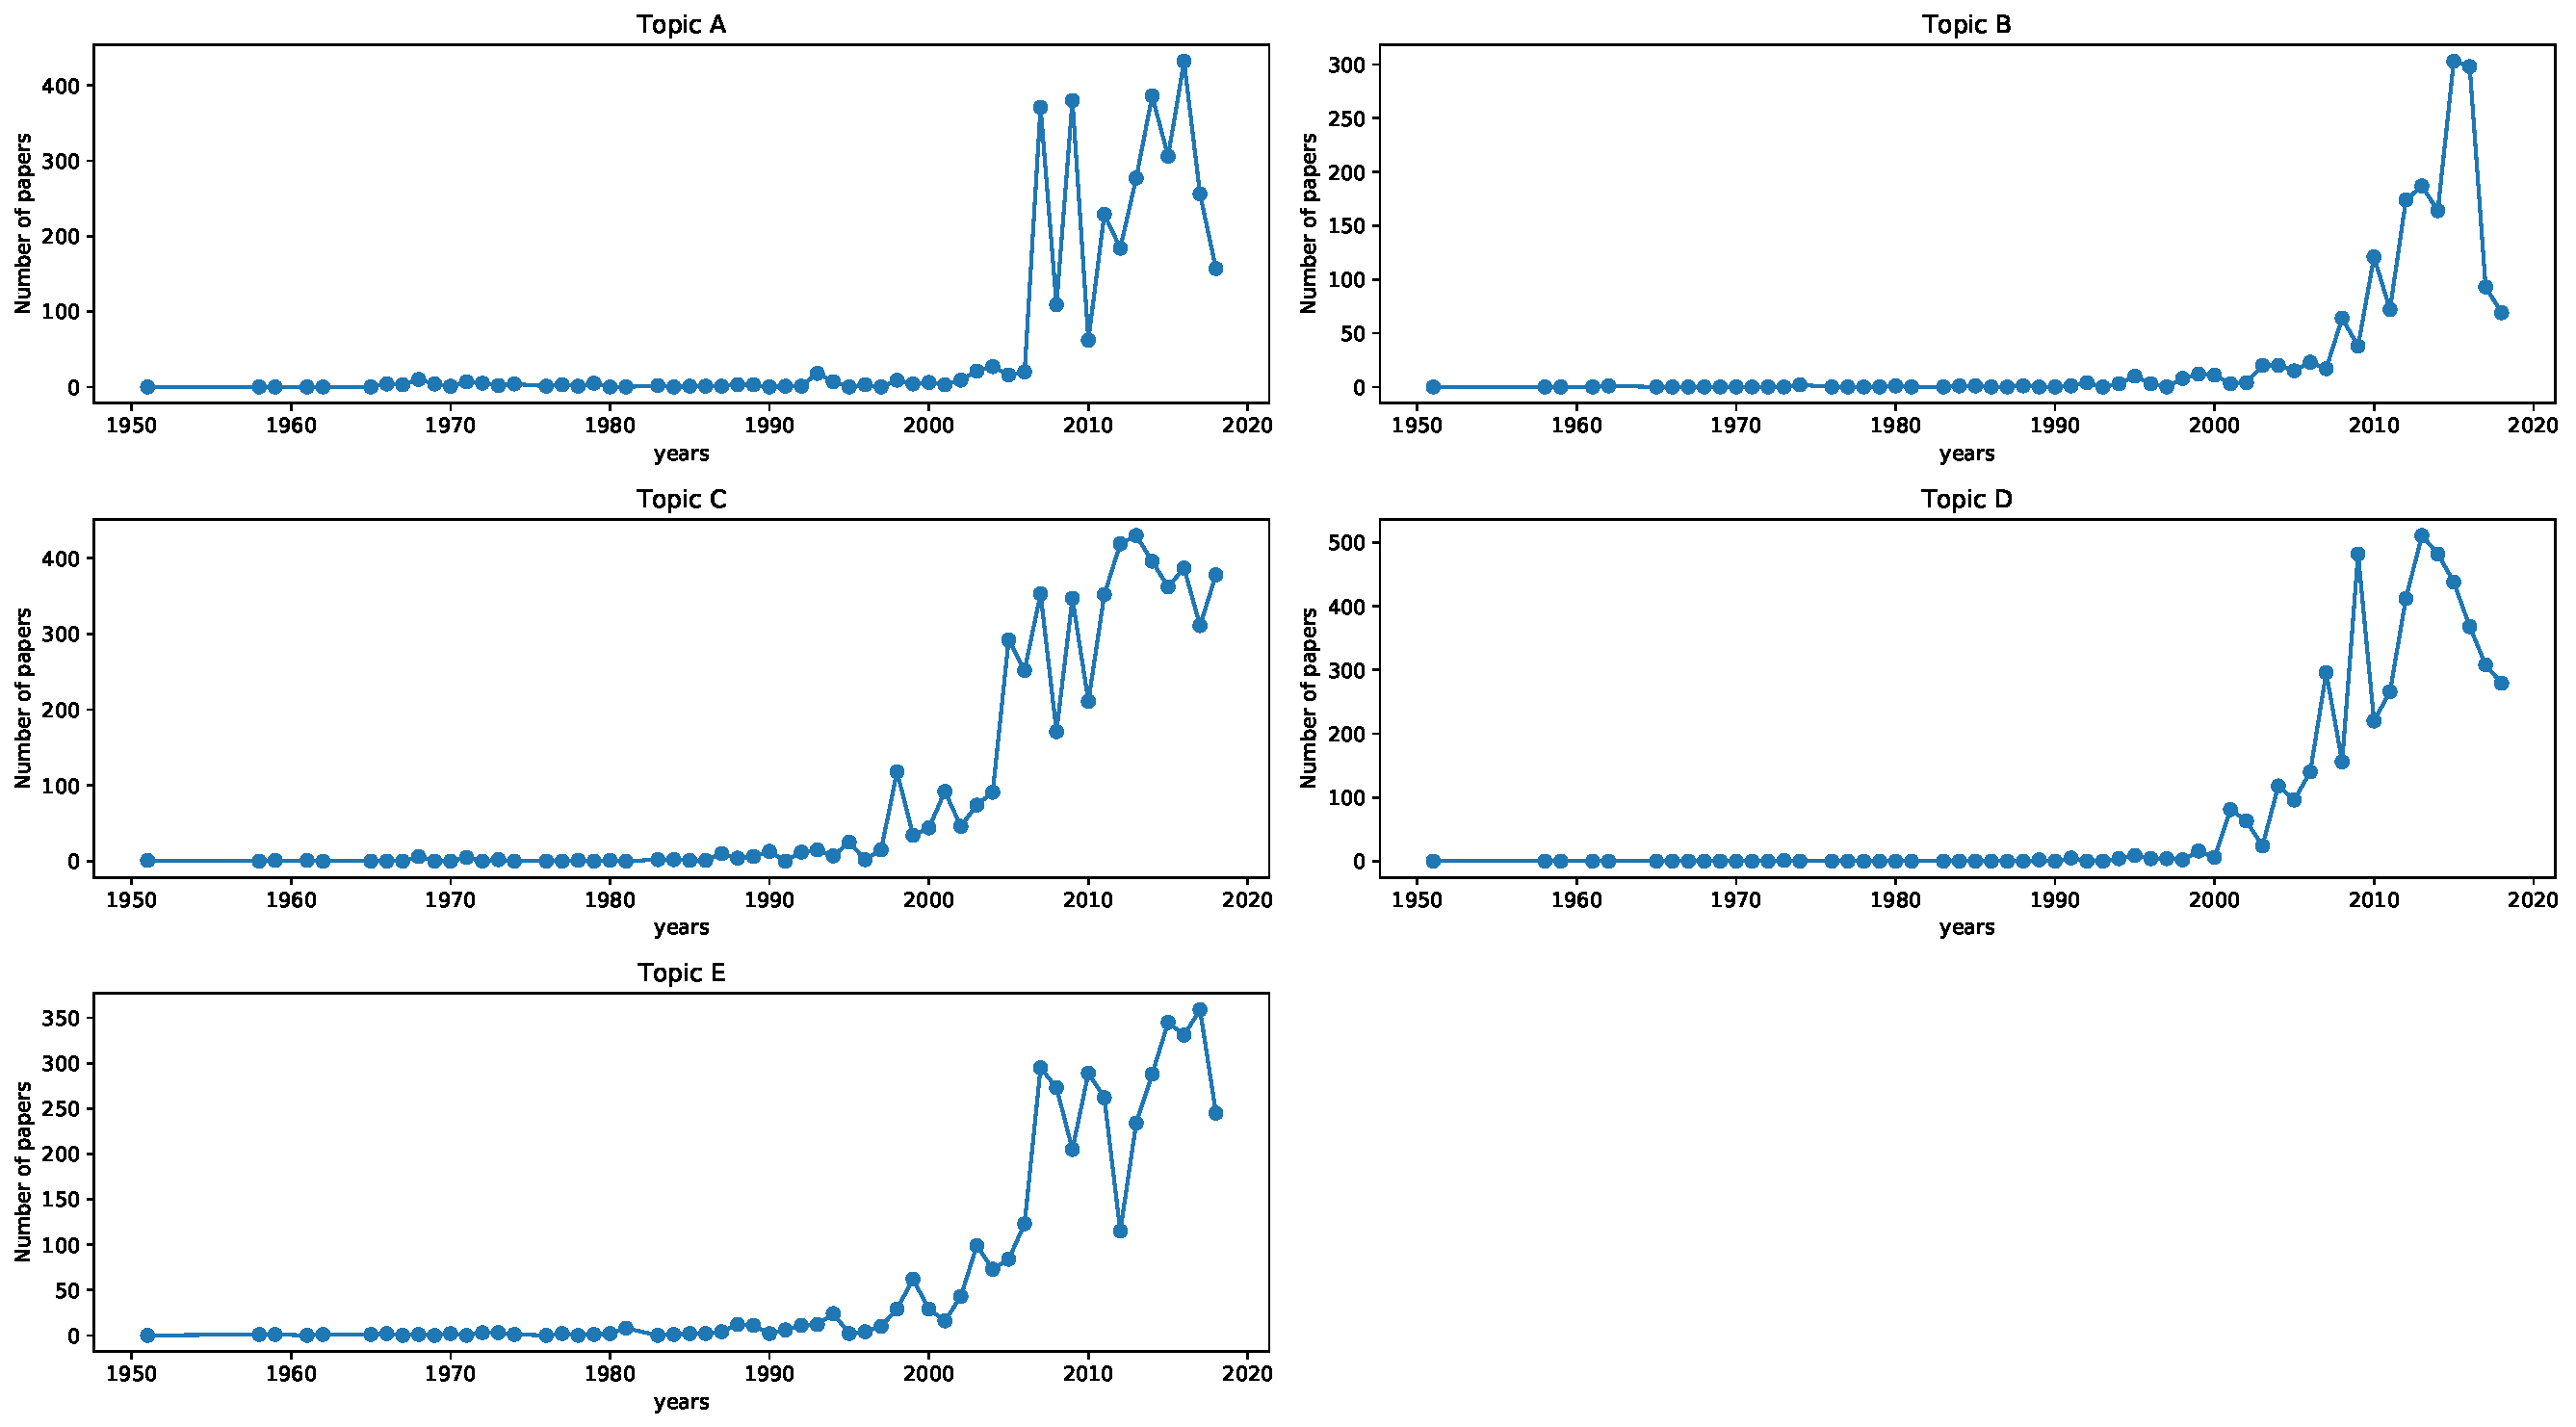
\includegraphics[width=\textwidth]{./assets/images/papers_per_topic_over_time.pdf}
    \caption{Number of articles per topic over the years.}\label{fig:number_of_articles_per_topic}
\end{figure}

To gain a better understanding regarding the number of topics over the years,
a topic modeling algorithm is applied to the cumulative data set over 8 periods.
These periods are 1951-1965, 1951-1973, 1951-1980, 1951-1988,
1951-1995, 1951-2003, 1951-2010, 1951-2018. The number of topics for each cumulative
subset is chosen based on the coherence value and only. The overlapping of keywords has
not been manually minimised. As a result, the period 1951-2018 has been assigned
6 topics instead of 5. Table~\ref{fig:number_of_articles_per_topic} gives the
topics, their keywords, the number of articles and their respective percentage
for each period. For period 1951 to 1965 the topics are labelled as 1 to 5
indicating that a total number of 5 topics was selected for that period.

There are several changes in the keywords over time, which is only natural as
the scientific language within a research field itself changes, and equivalently
the number of topics change as well. For example the word `sex', referring to
the male and female sex, does not appear in any keywords after 1988. This
implies that studying the effect of a participant's sex when playing an PD
became less frequently and possibly less important. The
word `evolution' is a keyword of topic 1 in the period 1951-1995. Topic 1 is
the largest topic of that period, implying that researchers were starting to
publish more on evolution. The word network is a keyword for the first time
following 2003. Suggesting that applications of the PD in social and computer
networks became more relevant after 2003.

\begin{table}[!hbtp]
    \begin{center}
    \resizebox{\textwidth}{!}{
    \begin{tabular}{llccc}
\toprule
    Period &  Topic &                                                                                                Topic Keywords & Num of Documents & Percentage of Documents \\
\midrule
 1951-1965 &               1 &                 problem, technology, divert, euler, subsystem, requirement, trace, technique, system, untried &                3 &                   0.375 \\
 1951-1965 &               2 &            interpret, requirement, programme, evolution, article, increase, policy, system, trace, technology &                2 &                    0.25 \\
 1951-1965 &               3 &          equipment, agency, conjecture, development, untried, programme, trend, technology, weapon, technique &                1 &                   0.125 \\
 1951-1965 &               4 &                 variation, celebrated, trend, untried, change, involve, month, technique, subsystem, research &                1 &                   0.125 \\
 1951-1965 &               5 &                           give, good, modern, trace, technique, ambiguity, problem, trend, technology, system &                1 &                   0.125 \\
 \midrule
 1951-1973 &               1 &                           study, shock, cooperative, money, part, vary, investigate, good, receive, equipment &               12 &                  0.3243 \\
 1951-1973 &               2 &          cooperation, level, significantly, sequence, reward, provoke, descriptive, principal, display, argue &                4 &                  0.1081 \\
 1951-1973 &               3 &               player, make, effect, triad, experimental, motivation, dominate, hypothesis, instruction, trend &                3 &                  0.0811 \\
 1951-1973 &               4 &                                           ss, sex, male, female, dyad, design, suggest, college, factor, tend &                3 &                  0.0811 \\
 1951-1973 &               5 &               result, research, format, change, operational, analysis, relate, understanding, decision, money &                2 &                  0.0541 \\
 1951-1973 &               6 &                          condition, give, high, treatment, conflict, cc, real, original, replication, promote &                2 &                  0.0541 \\
 1951-1973 &               7 &              group, competitive, show, interpret, scale, compete, escalation, free, variable, individualistic &                2 &                  0.0541 \\
 1951-1973 &               8 &                        outcome, strategy, choice, type, pdg, difference, dummy, conclude, compare, consistent &                2 &                  0.0541 \\
 1951-1973 &               9 &                   game, difference, pair, approach, behavior, person, weapon, occur, advantaged, differential &                2 &                  0.0541 \\
 1951-1973 &              10 &                    response, present, dilemma, influence, cooperate, bias, point, amount, participate, factor &                2 &                  0.0541 \\
 1951-1973 &              11 &                       trial, problem, previous, involve, prisoner, experiment, follow, tit, increase, initial &                1 &                   0.027 \\
 1951-1973 &              12 &                           matrix, behavior, rational, black, model, research, broad, distance, complex, trace &                1 &                   0.027 \\
 1951-1973 &              13 &                    play, finding, individual, noncooperative, white, nature, race, ratio, represent, prisoner &                1 &                   0.027 \\
 \midrule
 1951-1980 &               1 &                                      play, trial, group, follow, white, interpret, scale, black, trend, small &               14 &                    0.25 \\
 1951-1980 &               2 &                              outcome, level, effect, type, dyad, vary, pdg, participate, understanding, arise &                9 &                  0.1607 \\
 1951-1980 &               3 &         game, strategy, cooperation, significant, difference, sentence, text, occur, differential, hypothesis &                4 &                  0.0714 \\
 1951-1980 &               4 &                        male, female, find, result, sex, subject, experimental, situation, treatment, computer &                4 &                  0.0714 \\
 1951-1980 &               5 &                         research, problem, influence, matrix, format, model, analysis, year, crime, equipment &                4 &                  0.0714 \\
 1951-1980 &               6 &                                    condition, dilemma, bias, free, attempt, book, year, dummy, prison, design &                4 &                  0.0714 \\
 1951-1980 &               7 &                    variable, result, factor, individual, ability, triad, half, migration, change, investigate &                3 &                  0.0536 \\
 1951-1980 &               8 &                 show, present, suggest, rational, compete, approach, characteristic, examine, person, conduct &                3 &                  0.0536 \\
 1951-1980 &               9 &                         behavior, high, finding, relate, obtain, assistance, ratio, good, weapon, competition &                3 &                  0.0536 \\
 1951-1980 &              10 &                               ss, shock, money, competitive, part, difference, pair, amount, man, information &                3 &                  0.0536 \\
 1951-1980 &              11 &             player, conflict, theory, decision, determine, produce, maker, cooperate, specialist, programming &                2 &                  0.0357 \\
 1951-1980 &              12 &            study, prisoner, make, response, experiment, noncooperative, standard, separate, conclude, initial &                2 &                  0.0357 \\
 1951-1980 &              13 &                       give, cooperative, choice, cognitive, real, operational, set, subject, ascribe, concern &                1 &                  0.0179 \\
 \midrule
 1951-1988 &               1 &                     trial, difference, find, choice, significant, competitive, effect, triad, interact, occur &               24 &                  0.2553 \\
 1951-1988 &               2 &                                            ss, shock, money, pair, response, part, high, tit, receive, amount &               13 &                  0.1383 \\
 1951-1988 &               3 &                         suggest, paper, case, debate, view, achieve, framework, natural, assumption, finitely &               10 &                  0.1064 \\
 1951-1988 &               4 &                     prisoner, dilemma, behavior, model, present, involve, person, increase, trust, experiment &                8 &                  0.0851 \\
 1951-1988 &               5 &                                   game, player, show, approach, repeat, previous, move, tat, related, include &                8 &                  0.0851 \\
 1951-1988 &               6 &                cooperation, level, mutual, equilibrium, standard, provide, information, human, real, question &                6 &                  0.0638 \\
 1951-1988 &               7 &                      play, result, male, subject, female, cooperative, sex, experimental, treatment, computer &                5 &                  0.0532 \\
 1951-1988 &               8 &                        research, study, variable, ability, factor, conflict, matrix, year, student, interpret &                4 &                  0.0426 \\
 1951-1988 &               9 &                                         problem, group, small, scale, social, issue, large, base, bias, party &                4 &                  0.0426 \\
 1951-1988 &              10 &                          game, strategy, outcome, type, cooperate, ethical, pdg, explain, dependent, separate &                4 &                  0.0426 \\
 1951-1988 &              11 &              give, condition, individual, major, dyad, behaviour, produce, conflict, assistance, collectively &                3 &                  0.0319 \\
 1951-1988 &              12 &                        situation, iterate, statement, rational, card, side, paradox, true, consequence, front &                2 &                  0.0213 \\
 1951-1988 &              13 &                               inflation, hypothesis, rate, run, change, demand, nominal, cost, output, growth &                2 &                  0.0213 \\
 1951-1988 &              14 &                                     theory, make, analysis, decision, system, examine, work, soft, lead, hard &                1 &                  0.0106 \\
 \midrule
 1951-1995 &               1 &                            strategy, population, evolution, iterate, tit, opponent, evolve, dynamic, set, tat &               31 &                  0.1732 \\
 1951-1995 &               2 &                 game, repeat, assumption, rule, person, equilibrium, general, finitely, indefinitely, analyze &               24 &                  0.1341 \\
 1951-1995 &               3 &                            inflation, long, rate, hypothesis, run, policy, cost, nominal, demand, programming &               20 &                  0.1117 \\
 1951-1995 &               4 &            condition, outcome, trial, find, difference, cooperation, experiment, level, significant, response &               15 &                  0.0838 \\
 1951-1995 &               5 &                     rational, result, receive, statement, money, paradox, shock, iterate, consequence, common &               14 &                  0.0782 \\
 1951-1995 &               6 &             cooperation, show, competitive, high, probability, conflict, simulation, altruism, yield, natural &               14 &                  0.0782 \\
 1951-1995 &               7 &                           prisoner, dilemma, give, point, defect, form, cooperator, increase, relate, ethical &               10 &                  0.0559 \\
 1951-1995 &               8 &                       player, give, decision, provide, cooperative, game, previous, pair, determine, interact &                9 &                  0.0503 \\
 1951-1995 &               9 &                          play, cooperate, result, male, subject, female, time, relationship, suggest, student &                8 &                  0.0447 \\
 1951-1995 &              10 &                                   problem, group, theory, good, approach, society, large, scale, issue, level &                8 &                  0.0447 \\
 1951-1995 &              11 &            study, situation, behaviour, computer, argue, change, implication, characteristic, real, associate &                8 &                  0.0447 \\
 1951-1995 &              12 &                        model, paper, behavior, examine, present, mutual, expectation, develop, type, variable &                7 &                  0.0391 \\
 1951-1995 &              13 &                                   make, research, system, analysis, choice, work, base, relation, world, wide &                6 &                  0.0335 \\
 1951-1995 &              14 &               individual, social, behavior, standard, choose, evolutionary, partner, payoff, defection, small &                5 &                  0.0279 \\
 \midrule
 1951-2003 &               1 &                                    game, player, dilemma, prisoner, theory, give, paper, make, group, problem &              151 &                  0.4266 \\
 1951-2003 &               2 &                         cooperation, result, play, show, cooperate, condition, cooperative, high, level, time &              106 &                  0.2994 \\
 1951-2003 &               3 &                  strategy, model, agent, study, behavior, individual, population, evolutionary, state, player &               97 &                   0.274 \\
 \midrule
 1951-2010 &               1 &                                  model, theory, paper, base, make, present, problem, provide, human, decision &              325 &                  0.3454 \\
 1951-2010 &               2 &                                   game, strategy, player, agent, play, dilemma, system, behavior, show, state &              322 &                  0.3422 \\
 1951-2010 &               3 &  cooperation, network, study, population, individual, evolutionary, social, evolution, interaction, structure &              294 &                  0.3124 \\
 \midrule
 1951-2018 &               1 &                              model, theory, system, base, paper, problem, propose, present, approach, provide &              556 &                  0.2251 \\
 1951-2018 &               2 &                        behavior, social, human, decision, study, experiment, make, suggest, result, behaviour &              482 &                  0.1951 \\
 1951-2018 &               3 &                     individual, group, good, social, punishment, level, cost, mechanism, dilemma, cooperative &              428 &                  0.1733 \\
 1951-2018 &               4 &                            game, strategy, player, agent, play, dilemma, state, prisoner, payoff, equilibrium &              380 &                  0.1538 \\
 1951-2018 &               5 &                 population, evolutionary, dynamic, model, selection, result, evolution, evolve, show, process &              351 &                  0.1421 \\
 1951-2018 &               6 &       cooperation, network, interaction, structure, study, evolution, find, behavior, cooperative, simulation &              273 &                  0.1105 \\
\bottomrule
\end{tabular}
}
    \end{center}
    \caption{Topic modeling result for the cumulative data set over the periods
    }
\end{table}

In the following section the collaborative behaviour of authors in the field,
and within the field's topics as were presented in this section, are explored
using a network theoretic approach.

\section{Analysis of co-authorship network}\label{section:co_authorship}

In this section the collaborative behaviour of authors in the field of the IPD
is assessed using the co-authorship network. As mentioned in Section~\ref{section:methodology}
the co-authorship network is denoted as \(G\). There are a total of \connectedcomponents
connected components in \(G\) and the largest component has a size of 
\largestcc nodes. The largest connected component is going to be refereed to as
the main cluster of the network. The main cluster is denoted as \(\bar{G}\) and
a graphical representation is shown in Figure~\ref{fig:g_one_cluster}.
The metrics for both \(G\) and \(\bar{G}\) are given by
Table~\ref{table:network_comparison.tex}.


\begin{figure}[!hbtp]
    \begin{subfigure}{.45\textwidth}\centering
        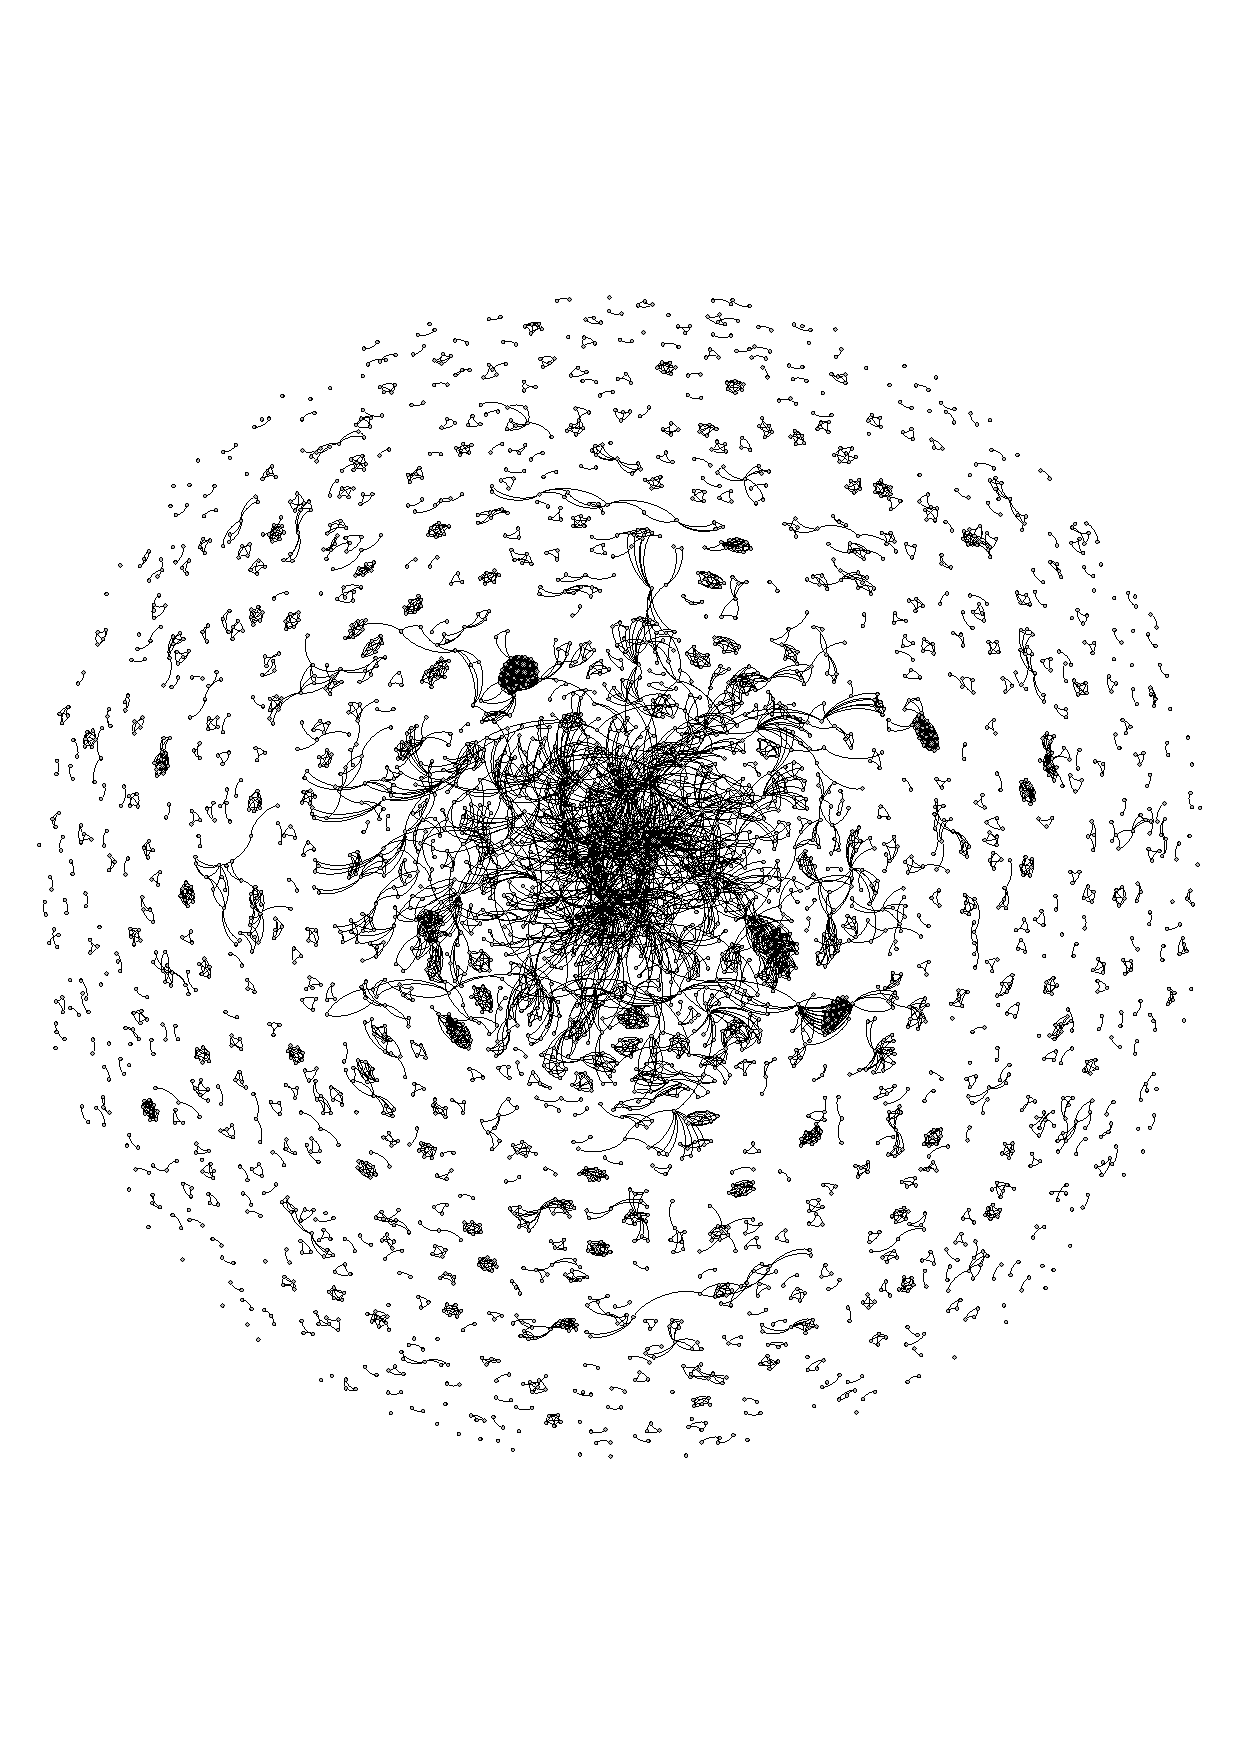
\includegraphics[width=.7\textwidth]{./assets/images/pd_network.pdf}
        \caption{\(G\) the co-authorship network for the IPD.}\label{fig:g_one_network}
    \end{subfigure}\hfill
    \begin{subfigure}{.45\textwidth}\centering
        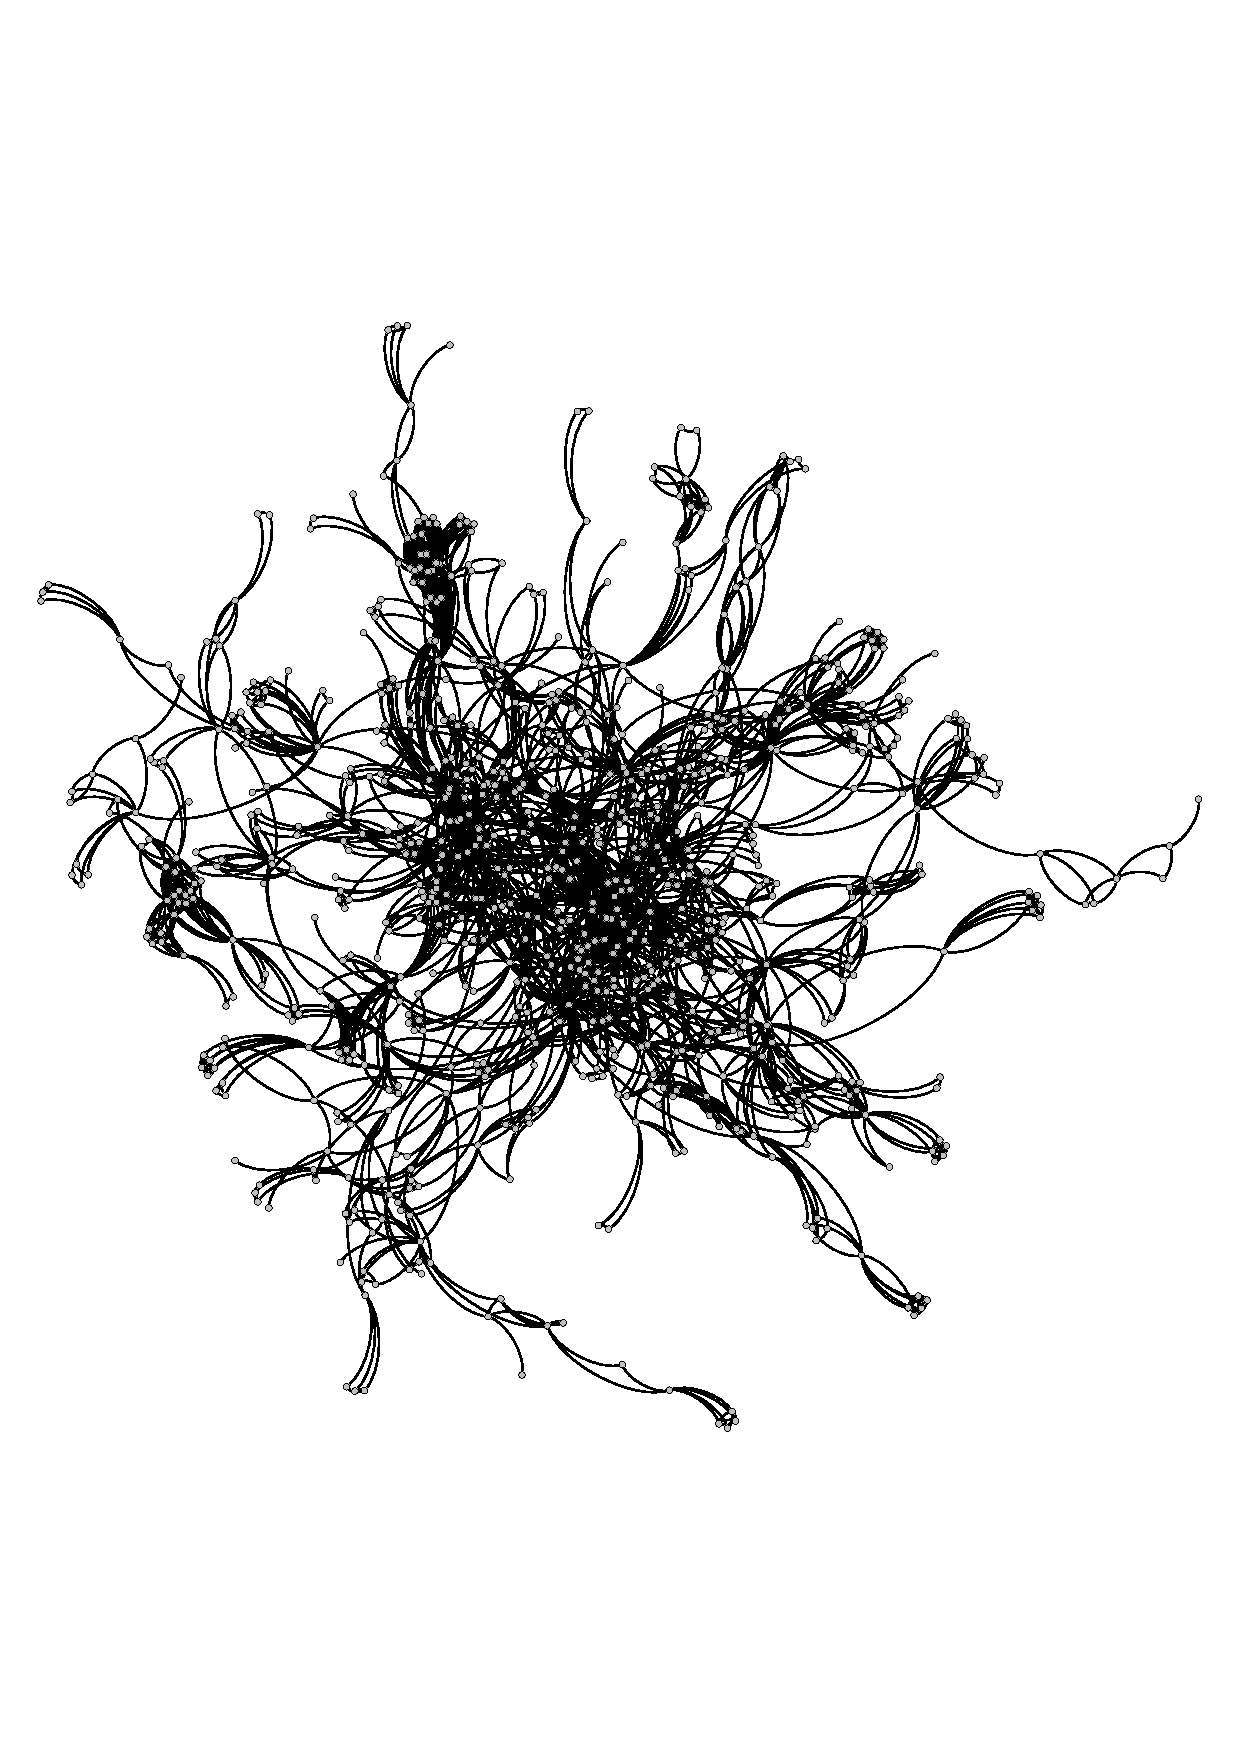
\includegraphics[width=.7\textwidth]{./assets/images/pd_network_cluster.pdf}
        \caption{\(\bar{G}\) the largest connected component of \(G\).}\label{fig:g_one_cluster}
     \end{subfigure}
\end{figure}

The networks have a high modularity and a large number of communities.
A high modularity implies that authors create their own publishing communities
but not many publications from authors from different communities occur.
However, the communities of the network are collaborative.
An author on average has 4 co-authors and 0.708 likelihood of collaborating
with a collaborator's co-author. There are only \isolated authors with single
author publications, which corresponds to only the \isolatedpercentage\% of authors
in \(G\). Moreover, in the PD an author from the main cluster is 7\% more
likely to write with a collaborator's co-author and on average has 2 more
co-authors.

In~\cite{Liu2015} the collaborative metrics for the ``evolution of cooperation''
co-authorship network were also reported. Though their network is of smaller
size (number of nodes 3670 \(<\) \authors), the collaborative metrics are fairly
similar between the two graphs (clustering coeff. \(0.632\) and modularity 0.95
close to 0.96), indicating that for the same field the same remarks can be made
from a different co-authorship network.

\begin{table}[!hbtp]
    \centering
    \resizebox{\textwidth}{!}{
    \begin{tabular}{lrrrrrrrrrr}
\toprule
{} &  \# Nodes &  \# Edges &  \# Isolated nodes &  \% Isolated nodes &  \# Connected components &  Size of largest component &  Av. degree &  \# Communities &  Modularity &  Clustering coeff \\
\midrule
$G$              &     4221 &     7642 &               338 &               8.0 &                    1157 &                        796 &       3.621 &           1177 &    0.965264 &             0.666 \\
$\bar{G}$        &      796 &     2214 &                 0 &               0.0 &                       1 &                        796 &       5.563 &             29 &    0.840138 &             0.773 \\
Auction Games    &     5362 &     7861 &               453 &               8.4 &                    1469 &                       1348 &       2.932 &           1493 &    0.957238 &             0.599 \\
Price of Anarchy &     1315 &     1952 &               165 &              12.5 &                     406 &                        221 &       2.969 &            414 &    0.964498 &             0.626 \\
\bottomrule
\end{tabular}
}
    \caption{Network metrics for \(G\) and \(\bar{G}\) respectively.}
    \label{table:network_comparison.tex}
\end{table}

The change of the network over time is also studied by constructing the network
cumulatively over 51 periods. Except from the first period 1951-1966 the rest of
the periods have a yearly interval (data for the years 1975 and 1982 have not
been collected). The metrics of each sub network are given by
Table~\ref{table:coll_cumulative}. This is also done for \(\bar{G}\) over the
same periods and the results are given by Table~\ref{table:clusters_cumulative}.
Similar to the results of~\cite{Liu2015}, it can been observed that the network
\(G\) grows over time and that the network always has modularity. This is also
confirmed by \(\bar{G}\).

\begin{table}[!hbtp]
    \centering
    \resizebox{\textwidth}{!}{
    \begin{tabular}{lrrrrrrrllr}
\toprule
{} &  \# Nodes &  \# Edges &  \# Isolated nodes &  \% Isolated nodes &  \# Connected components &  Size of largest component &  Av. degree & \# Communities & Modularity &  Clustering coeff \\
\midrule
1954 - 1950 &        3 &        0 &                 3 &             100.0 &                       3 &                          1 &       0.000 &             - &          - &             0.000 \\
1954 - 1955 &        2 &        0 &                 2 &             100.0 &                       2 &                          1 &       0.000 &             - &          - &             0.000 \\
1955 - 1956 &        3 &        0 &                 3 &             100.0 &                       3 &                          1 &       0.000 &             - &          - &             0.000 \\
1956 - 1957 &        4 &        0 &                 4 &             100.0 &                       4 &                          1 &       0.000 &             - &          - &             0.000 \\
1957 - 1958 &        6 &        0 &                 6 &             100.0 &                       6 &                          1 &       0.000 &             - &          - &             0.000 \\
1958 - 1959 &        7 &        0 &                 7 &             100.0 &                       7 &                          1 &       0.000 &             - &          - &             0.000 \\
1959 - 1961 &        7 &        0 &                 7 &             100.0 &                       7 &                          1 &       0.000 &             - &          - &             0.000 \\
1961 - 1962 &        8 &        0 &                 8 &             100.0 &                       8 &                          1 &       0.000 &             - &          - &             0.000 \\
1962 - 1964 &        9 &        0 &                 9 &             100.0 &                       9 &                          1 &       0.000 &             - &          - &             0.000 \\
1964 - 1965 &       10 &        0 &                10 &             100.0 &                      10 &                          1 &       0.000 &             - &          - &             0.000 \\
1965 - 1966 &       17 &        3 &                11 &              64.7 &                      14 &                          2 &       0.353 &            14 &   0.666667 &             0.000 \\
1966 - 1967 &       21 &        4 &                13 &              61.9 &                      17 &                          2 &       0.381 &            17 &       0.75 &             0.000 \\
1967 - 1968 &       32 &       15 &                13 &              40.6 &                      21 &                          5 &       0.938 &            21 &   0.684444 &             0.135 \\
1968 - 1969 &       36 &       17 &                16 &              44.4 &                      24 &                          6 &       0.944 &            24 &   0.629758 &             0.139 \\
1969 - 1970 &       39 &       18 &                17 &              43.6 &                      26 &                          6 &       0.923 &            26 &   0.666667 &             0.128 \\
1970 - 1971 &       51 &       28 &                18 &              35.3 &                      31 &                          6 &       1.098 &            31 &   0.826531 &             0.275 \\
1971 - 1972 &       58 &       34 &                19 &              32.8 &                      34 &                          6 &       1.172 &            34 &   0.866782 &             0.345 \\
1972 - 1973 &       59 &       35 &                18 &              30.5 &                      34 &                          6 &       1.186 &            34 &   0.873469 &             0.339 \\
1973 - 1974 &       59 &       35 &                18 &              30.5 &                      34 &                          6 &       1.186 &            34 &   0.873469 &             0.339 \\
1974 - 1975 &       60 &       35 &                19 &              31.7 &                      35 &                          6 &       1.167 &            35 &   0.873469 &             0.333 \\
1975 - 1976 &       60 &       35 &                19 &              31.7 &                      35 &                          6 &       1.167 &            35 &   0.873469 &             0.333 \\
1976 - 1977 &       68 &       37 &                23 &              33.8 &                      41 &                          6 &       1.088 &            41 &   0.885318 &             0.294 \\
1977 - 1978 &       70 &       38 &                23 &              32.9 &                      42 &                          6 &       1.086 &            42 &   0.890582 &             0.286 \\
1978 - 1979 &       73 &       42 &                23 &              31.5 &                      42 &                          6 &       1.151 &            42 &   0.893424 &             0.292 \\
1979 - 1980 &       77 &       45 &                25 &              32.5 &                      44 &                          6 &       1.169 &            44 &   0.899753 &             0.307 \\
1980 - 1981 &       80 &       50 &                26 &              32.5 &                      45 &                          6 &       1.250 &            45 &     0.8928 &             0.318 \\
1981 - 1982 &       84 &       56 &                26 &              31.0 &                      46 &                          6 &       1.333 &            46 &   0.903061 &             0.350 \\
1982 - 1983 &       87 &       57 &                27 &              31.0 &                      48 &                          6 &       1.310 &            48 &   0.906125 &             0.338 \\
1983 - 1984 &       94 &       58 &                32 &              34.0 &                      54 &                          6 &       1.234 &            54 &   0.909037 &             0.313 \\
1984 - 1985 &       95 &       58 &                33 &              34.7 &                      55 &                          6 &       1.221 &            55 &   0.909037 &             0.309 \\
1985 - 1986 &      104 &       59 &                40 &              38.5 &                      63 &                          6 &       1.135 &            63 &   0.911807 &             0.283 \\
1986 - 1987 &      116 &       61 &                48 &              41.4 &                      73 &                          6 &       1.052 &            73 &   0.916958 &             0.253 \\
1987 - 1988 &      121 &       65 &                48 &              39.7 &                      75 &                          6 &       1.074 &            75 &   0.924497 &             0.268 \\
1988 - 1989 &      134 &       76 &                47 &              35.1 &                      80 &                          6 &       1.134 &            80 &   0.937673 &             0.272 \\
1989 - 1990 &      145 &       82 &                49 &              33.8 &                      86 &                          6 &       1.131 &            86 &   0.944676 &             0.272 \\
1990 - 1991 &      158 &       88 &                53 &              33.5 &                      94 &                          6 &       1.114 &            94 &   0.950413 &             0.268 \\
1991 - 1992 &      169 &       91 &                59 &              34.9 &                     102 &                          6 &       1.077 &           102 &   0.953025 &             0.251 \\
1992 - 1993 &      186 &      104 &                62 &              33.3 &                     110 &                          6 &       1.118 &           110 &    0.95932 &             0.266 \\
1993 - 1994 &      220 &      134 &                72 &              32.7 &                     127 &                          6 &       1.218 &           127 &   0.965471 &             0.317 \\
1994 - 1995 &      239 &      144 &                74 &              31.0 &                     137 &                          6 &       1.205 &           137 &   0.969329 &             0.304 \\
1995 - 1996 &      257 &      163 &                77 &              30.0 &                     145 &                          6 &       1.268 &           145 &   0.970831 &             0.318 \\
1996 - 1997 &      279 &      178 &                81 &              29.0 &                     156 &                          6 &       1.276 &           156 &   0.974309 &             0.336 \\
1997 - 1998 &      311 &      215 &                65 &              20.9 &                     160 &                          6 &       1.383 &           160 &   0.979773 &             0.354 \\
1998 - 1999 &      329 &      239 &                58 &              17.6 &                     162 &                          6 &       1.453 &           162 &   0.981741 &             0.376 \\
1999 - 2000 &      373 &      273 &                67 &              18.0 &                     183 &                          6 &       1.464 &           183 &   0.983778 &             0.387 \\
2000 - 2001 &      400 &      320 &                54 &              13.5 &                     184 &                          7 &       1.600 &           184 &   0.983066 &             0.410 \\
2001 - 2002 &      450 &      366 &                61 &              13.6 &                     206 &                          7 &       1.627 &           206 &   0.984547 &             0.418 \\
2002 - 2003 &      509 &      414 &                58 &              11.4 &                     229 &                          7 &       1.627 &           229 &   0.987083 &             0.421 \\
2003 - 2004 &      580 &      489 &                58 &              10.0 &                     253 &                         10 &       1.686 &           253 &   0.988052 &             0.429 \\
2004 - 2005 &      679 &      599 &                57 &               8.4 &                     284 &                         19 &       1.764 &           284 &    0.98891 &             0.463 \\
2005 - 2006 &      854 &      806 &                66 &               7.7 &                     342 &                         21 &       1.888 &           342 &   0.990724 &             0.496 \\
2006 - 2007 &     1056 &     1117 &                76 &               7.2 &                     402 &                         24 &       2.116 &           402 &   0.989663 &             0.527 \\
2007 - 2008 &     1255 &     1460 &                85 &               6.8 &                     454 &                         32 &       2.327 &           455 &   0.989753 &             0.549 \\
2008 - 2009 &     1462 &     1759 &               104 &               7.1 &                     520 &                         56 &       2.406 &           521 &   0.987517 &             0.550 \\
2009 - 2010 &     1700 &     2301 &               114 &               6.7 &                     581 &                         99 &       2.707 &           584 &   0.979084 &             0.571 \\
2010 - 2011 &     2040 &     2954 &               121 &               5.9 &                     665 &                        121 &       2.896 &           668 &   0.980477 &             0.603 \\
2011 - 2012 &     2422 &     3676 &               126 &               5.2 &                     756 &                        210 &       3.036 &           759 &   0.979196 &             0.629 \\
2012 - 2013 &     2807 &     4398 &               138 &               4.9 &                     843 &                        330 &       3.134 &           849 &   0.976132 &             0.639 \\
2013 - 2014 &     3199 &     5044 &               148 &               4.6 &                     942 &                        406 &       3.153 &           950 &   0.974968 &             0.651 \\
2014 - 2015 &     3798 &     6221 &               159 &               4.2 &                    1064 &                        514 &       3.276 &          1074 &   0.976242 &             0.668 \\
2015 - 2016 &     4472 &     8344 &               169 &               3.8 &                    1184 &                        614 &       3.732 &          1198 &   0.975233 &             0.690 \\
2016 - 2017 &     4925 &     9235 &               173 &               3.5 &                    1274 &                        703 &       3.750 &          1292 &   0.976353 &             0.700 \\
2017 - 2018 &     5385 &    10379 &               176 &               3.3 &                    1356 &                        815 &       3.855 &          1369 &   0.977318 &             0.708 \\
\bottomrule
\end{tabular}
}
    \caption{Collaborativeness metrics for cumulative graphs, \(\tilde{G} \subseteq G\).}\label{table:coll_cumulative}
\end{table}

\begin{table}[!hbtp]
    \centering
    \resizebox{\textwidth}{!}{
    \begin{tabular}{lrrrrrrrrrr}
\toprule
Periods &  \# Nodes &  \# Edges &  \# Isolated nodes &  \% Isolated nodes &  \# Connected components &  Size of largest component &  Av. degree &  \# Communities &  Modularity &  Clustering coeff \\
\midrule
1951 - 1966 &        2 &        1 &                 0 &               0.0 &                       1 &                          2 &       1.000 &              1 &       0.000 &             0.000 \\
1951 - 1967 &        2 &        1 &                 0 &               0.0 &                       1 &                          2 &       1.000 &              1 &       0.000 &             0.000 \\
1951 - 1968 &        5 &        8 &                 0 &               0.0 &                       1 &                          5 &       3.200 &              1 &       0.000 &             0.867 \\
1951 - 1969 &        6 &       10 &                 0 &               0.0 &                       1 &                          6 &       3.333 &              2 &       0.020 &             0.833 \\
1951 - 1970 &        6 &       10 &                 0 &               0.0 &                       1 &                          6 &       3.333 &              2 &       0.020 &             0.833 \\
1951 - 1971 &        6 &       10 &                 0 &               0.0 &                       1 &                          6 &       3.333 &              2 &       0.020 &             0.833 \\
1951 - 1972 &        6 &       10 &                 0 &               0.0 &                       1 &                          6 &       3.333 &              2 &       0.020 &             0.833 \\
1951 - 1973 &        6 &       10 &                 0 &               0.0 &                       1 &                          6 &       3.333 &              2 &       0.020 &             0.833 \\
1951 - 1974 &        6 &       10 &                 0 &               0.0 &                       1 &                          6 &       3.333 &              2 &       0.020 &             0.833 \\
1951 - 1976 &        6 &       10 &                 0 &               0.0 &                       1 &                          6 &       3.333 &              2 &       0.020 &             0.833 \\
1951 - 1977 &        6 &       10 &                 0 &               0.0 &                       1 &                          6 &       3.333 &              2 &       0.020 &             0.833 \\
1951 - 1978 &        6 &       10 &                 0 &               0.0 &                       1 &                          6 &       3.333 &              2 &       0.020 &             0.833 \\
1951 - 1979 &        6 &       10 &                 0 &               0.0 &                       1 &                          6 &       3.333 &              2 &       0.020 &             0.833 \\
1951 - 1980 &        6 &       10 &                 0 &               0.0 &                       1 &                          6 &       3.333 &              2 &       0.020 &             0.833 \\
1951 - 1981 &        6 &       10 &                 0 &               0.0 &                       1 &                          6 &       3.333 &              2 &       0.020 &             0.833 \\
1951 - 1983 &        6 &       10 &                 0 &               0.0 &                       1 &                          6 &       3.333 &              2 &       0.020 &             0.833 \\
1951 - 1984 &        6 &       10 &                 0 &               0.0 &                       1 &                          6 &       3.333 &              2 &       0.020 &             0.833 \\
1951 - 1985 &        6 &       10 &                 0 &               0.0 &                       1 &                          6 &       3.333 &              2 &       0.020 &             0.833 \\
1951 - 1986 &        6 &       10 &                 0 &               0.0 &                       1 &                          6 &       3.333 &              2 &       0.020 &             0.833 \\
1951 - 1987 &        6 &       10 &                 0 &               0.0 &                       1 &                          6 &       3.333 &              2 &       0.020 &             0.833 \\
1951 - 1988 &        6 &       10 &                 0 &               0.0 &                       1 &                          6 &       3.333 &              2 &       0.020 &             0.833 \\
1951 - 1989 &        6 &       10 &                 0 &               0.0 &                       1 &                          6 &       3.333 &              2 &       0.020 &             0.833 \\
1951 - 1990 &        6 &       10 &                 0 &               0.0 &                       1 &                          6 &       3.333 &              2 &       0.020 &             0.833 \\
1951 - 1991 &        6 &       10 &                 0 &               0.0 &                       1 &                          6 &       3.333 &              2 &       0.020 &             0.833 \\
1951 - 1992 &        6 &       10 &                 0 &               0.0 &                       1 &                          6 &       3.333 &              2 &       0.020 &             0.833 \\
1951 - 1993 &        6 &       10 &                 0 &               0.0 &                       1 &                          6 &       3.333 &              2 &       0.020 &             0.833 \\
1951 - 1994 &        6 &       10 &                 0 &               0.0 &                       1 &                          6 &       3.333 &              2 &       0.020 &             0.833 \\
1951 - 1995 &        6 &       10 &                 0 &               0.0 &                       1 &                          6 &       3.333 &              2 &       0.020 &             0.833 \\
1951 - 1996 &        6 &       10 &                 0 &               0.0 &                       1 &                          6 &       3.333 &              2 &       0.020 &             0.833 \\
1951 - 1997 &        6 &       10 &                 0 &               0.0 &                       1 &                          6 &       3.333 &              2 &       0.020 &             0.833 \\
1951 - 1998 &        6 &       10 &                 0 &               0.0 &                       1 &                          6 &       3.333 &              2 &       0.020 &             0.833 \\
1951 - 1999 &        6 &       10 &                 0 &               0.0 &                       1 &                          6 &       3.333 &              2 &       0.020 &             0.833 \\
1951 - 2000 &        6 &       10 &                 0 &               0.0 &                       1 &                          6 &       3.333 &              2 &       0.020 &             0.833 \\
1951 - 2001 &        7 &       21 &                 0 &               0.0 &                       1 &                          7 &       6.000 &              1 &       0.000 &             1.000 \\
1951 - 2002 &        7 &       21 &                 0 &               0.0 &                       1 &                          7 &       6.000 &              1 &       0.000 &             1.000 \\
1951 - 2003 &        7 &       21 &                 0 &               0.0 &                       1 &                          7 &       6.000 &              1 &       0.000 &             1.000 \\
1951 - 2004 &       10 &       13 &                 0 &               0.0 &                       1 &                         10 &       2.600 &              2 &       0.376 &             0.553 \\
1951 - 2005 &       19 &       28 &                 0 &               0.0 &                       1 &                         19 &       2.947 &              3 &       0.544 &             0.730 \\
1951 - 2006 &       22 &       35 &                 0 &               0.0 &                       1 &                         22 &       3.182 &              4 &       0.527 &             0.720 \\
1951 - 2007 &       25 &       39 &                 0 &               0.0 &                       1 &                         25 &       3.120 &              5 &       0.558 &             0.686 \\
1951 - 2008 &       33 &       62 &                 0 &               0.0 &                       1 &                         33 &       3.758 &              4 &       0.623 &             0.736 \\
1951 - 2009 &       71 &      148 &                 0 &               0.0 &                       1 &                         71 &       4.169 &              6 &       0.697 &             0.698 \\
1951 - 2010 &      133 &      387 &                 0 &               0.0 &                       1 &                        133 &       5.820 &              7 &       0.726 &             0.749 \\
1951 - 2011 &      157 &      465 &                 0 &               0.0 &                       1 &                        157 &       5.924 &              8 &       0.727 &             0.725 \\
1951 - 2012 &      209 &      611 &                 0 &               0.0 &                       1 &                        209 &       5.847 &             11 &       0.733 &             0.737 \\
1951 - 2013 &      322 &      892 &                 0 &               0.0 &                       1 &                        322 &       5.540 &             12 &       0.780 &             0.743 \\
1951 - 2014 &      399 &     1109 &                 0 &               0.0 &                       1 &                        399 &       5.559 &             15 &       0.794 &             0.742 \\
1951 - 2015 &      504 &     1368 &                 0 &               0.0 &                       1 &                        504 &       5.429 &             24 &       0.811 &             0.751 \\
1951 - 2016 &      613 &     1677 &                 0 &               0.0 &                       1 &                        613 &       5.471 &             21 &       0.819 &             0.761 \\
1951 - 2017 &      706 &     1935 &                 0 &               0.0 &                       1 &                        706 &       5.482 &             29 &       0.830 &             0.772 \\
1951 - 2018 &      796 &     2214 &                 0 &               0.0 &                       1 &                        796 &       5.563 &             25 &       0.845 &             0.773 \\
\bottomrule
\end{tabular}
}
    \caption{Collaborativeness metrics for cumulative graphs' main clusters, \(\tilde{G} \subseteq \bar{G}\).}\label{table:clusters_cumulative}
\end{table}

In Section~\ref{section:results} the articles of this work were classified into
5 different topics. The co-authorship networks for each topic have been
constructed in the same way as \(G\). Note that authors with publications in more
than one topic exist. These authors have not been removed.
The metrics of the five co-authorship networks are given
by Table~\ref{table:topics_networks}.

Though Topic B has the smallest number of articles and is the smallest network
as well, with 695 authors, it has the highest average degree.
The network of Topic A is the largest network, moreover, it has the smallest
percentage of isolated nodes (1.3\%) and an average degree of 3.8. The networks
of topics E and C have a large number of isolated nodes, 5.9\% and 4.6\%
respectively, a small clustering coefficient and Topic C has the smallest
average degree. The authors with publications in Topics B and A appear be more
collaborative, with authors having 4 co-authors and hardly writing at all,
compared to Topics E and C. Topic D has the largest connected component though
it is one of the smallest networks. The connected component of topic D is made
up by the same authors as the main cluster \(\bar{G}\), this will be clear in
the next result.

\begin{table}[H]
    \centering
    \resizebox{\textwidth}{!}{
    \begin{tabular}{lrrrrrrrrrr}
\toprule
{} &  \# Nodes &  \# Edges &  \# Isolated nodes &  \% Isolated nodes &  \# Connected components &  Size of largest component &  Av. degree &  \# Communities &  Modularity &  Clustering coeff \\
\midrule
Topic A &     1124 &     2137 &                15 &               1.3 &                     264 &                         56 &       3.802 &            265 &       0.983 &             0.759 \\
Topic B &      695 &     1382 &                13 &               1.9 &                     157 &                         80 &       3.977 &            158 &       0.950 &             0.773 \\
Topic C &      900 &     1141 &                41 &               4.6 &                     281 &                         29 &       2.536 &            281 &       0.981 &             0.636 \\
Topic D &      880 &     1509 &                17 &               1.9 &                     174 &                        312 &       3.430 &            183 &       0.918 &             0.701 \\
Topic E &     1045 &     1964 &                59 &               5.6 &                     354 &                         31 &       3.759 &            354 &       0.926 &             0.664 \\
\bottomrule
\end{tabular}
}
    \caption{Network metrics for topic networks.}\label{table:topics_networks}
\end{table}

Though the authors with publications in topics C, D and E have exhibited to be
less collaborative it must be taken into account that authors had their
publications assigned to multiple topics, and thus the edges of a node have been
divided between the different networks. More specifically, a total of 1975
authors have articles assigned to multiple topics. Out of these 1975 authors,
55\% of them had their publications assigned to two different topics, 30\% in
three, 10\% in four and 5\% in five,
Figure~\ref{fig:different_topics_per_author}. The probabilities of having
publications being assigned to a given combination of topics based on the
different number of topics are given by Table~\ref{table:topic_probabilities}.
Table~\ref{table:topic_probabilities} shows that authors are most likely to have
their publications assigned to topics C and D, C and E (for \(n=2\)), C, D and E
(for \(n=3\)) and A, C, D and E (for \(n=4\)). Indeed the authors with
publications in topics C, D and E could have suffered from their connections
being divided into different networks, and thus the respective networks could be
more collaborative than the analysis has suggested.


\begin{figure}[!hbtp]
    \centering
    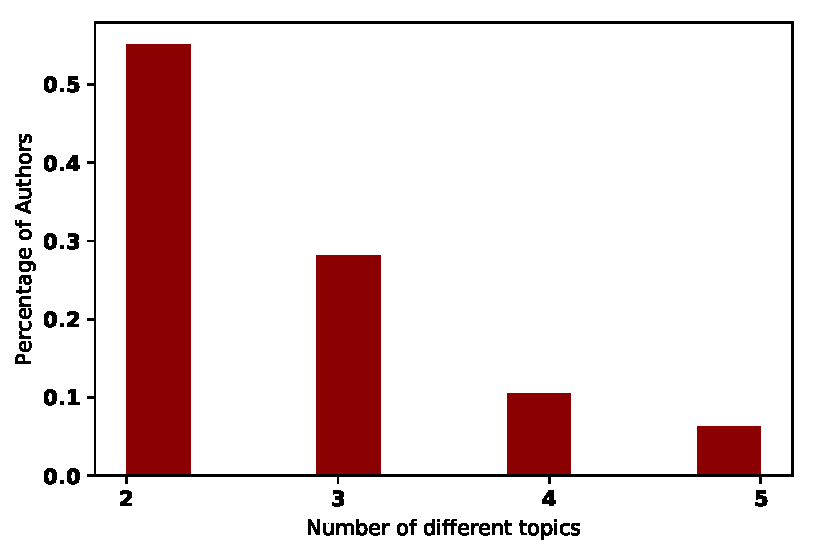
\includegraphics[width=.45\textwidth]{./assets/images/percentage_of_authors_different_topic.pdf}
    \caption{Distribution of number of different topics authors have written in
    excluding single topic.}
    \label{fig:different_topics_per_author}
\end{figure}

\begin{table}[!htbp]
    \begin{center}
    \resizebox{.55\textwidth}{!}{\begin{tabular}{clr}
\toprule
Number of different topics authors have publications \(n\) &  Topics &  Probabilities \\
\midrule
\(n = 2\)&                  B - E &           0.04 \\
&                  C - D &           0.24 \\
&                  C - E &           0.15 \\
&                  A - B &           0.08 \\
&                  D - E &           0.13 \\
&                  A - E &           0.07 \\
&                  B - C &           0.03 \\
&                  B - D &           0.07 \\
&                  A - D &           0.12 \\
&                  A - C &           0.07 \\
\midrule
\(n = 3\)&              A - D - E &           0.10 \\
&              C - D - E &           0.29 \\
&              A - B - C &           0.04 \\
&              A - C - D &           0.13 \\
&              B - C - D &           0.11 \\
&              A - B - E &           0.03 \\
&              A - B - D &           0.10 \\
&              B - C - E &           0.04 \\
&              A - C - E &           0.09 \\
&              B - D - E &           0.06 \\
\midrule
\(n = 4\)&          A - C - D - E &           0.35 \\
&          A - B - C - D &           0.14 \\
&          B - C - D - E &           0.33 \\
&          A - B - D - E &           0.13 \\
&          A - B - C - E &           0.06 \\
\midrule
\(n = 5\)&      A - B - C - D - E &           1.00 \\
\bottomrule
\end{tabular}
}
\end{center}
\caption{Probabilities of an author writing in any combinations of
topics based on the number of topics the author has publications in.}\label{table:topic_probabilities}
\end{table}

The next result discussed here are on centrality measures. As a reminder, two
centrality measures are reported, these are the closeness centrality and the
betweenness centrality. Closeness centrality is a measure of how easy it is for
an author to contact others, and consequently affect them; influence them. Thus
closeness centrality here is a measure of influence. Betweenness centrality is a
measure of how many paths pass through a specific node, thus the amount of
information this person has access to. Betweenness centrality is used here as a
measure of how much an author gains from the field. All centrality measure can
have values ranging from 0 to 1.

For \(G\) and \(\bar{G}\) the most central authors based on closeness and
betweenness centralities are given by Table~\ref{table:central_authors}. For \(G\) the
most central author, based on both measures, is Matjaz Perc. A
few authors appear to be central based on one measure and not the other. Martin
Nowak, Franz Weissing, Jianye Hao, Angel Sanchez and Valerio Capraro are authors
that have access to information due to their positioning but do not
influence the network as much. The opposite is true for the authors Attila
Szolnoki, Luo-Luo Jiang Sandro Meloni, Cheng-Yi Xia and Xiaojie Chen.
Overall the values of both measures are low. The medians of the distributions, given
in Figures~\ref{fig:bc_distributions} and~\ref{fig:cc_distributions}, are both zero.
From Figure~\ref{fig:cc_distributions} it is evident that some authors have
higher values of closeness centrality and thus do influence the network. These can be
verified to be the authors from the main cluster. The most central authors
in \(\bar{G}\) are the same people as in \(G\). This implies that
the results on centrality heavily rely of the main cluster.

In conclusion the authors of the PD do not gain much from the influence of their
fields. This can even be verified by the topics networks. Table~\ref{table:central_authors_bc_topics}
the authors that gain the most from their respective topics and the values are
once again low. In some cases even zero (Topic A, C and E).
In relation to authors influencing their field. There are authors in \(G\) that
do influence the network. The group of people that do are the authors of
the main cluster. These authors even gain from being in the main cluster and
part of this "main" group of authors. From Table~\ref{table:central_authors_cc_topics}
it can be seen that Topic D
has the highest values of closeness centrality and this is because the authors
are a subset of \(\bar{G}\). In comparison the other networks have very low
values of centrality and the results are verified further by the topics' networks.

% The distributions of the centralities over the topics are given
% in Figures~\ref{fig:bc_distributions_topics} and~\ref{fig:bc_distributions_topics}.

\begin{table}[!hbtp]
    \begin{center}
    \resizebox{.9\textwidth}{!}{\begin{tabular}{llrlrlrlr}
\toprule
& \multicolumn{4}{c}{$G$} & \multicolumn{4}{c}{$\bar{G}$} \\
\midrule
{} &             Name &  Betweenness &             Name &  Closeness &             Name &  Betweenness &             Name &  Closeness \\
\midrule
1  &      Matjaz Perc &        0.013 &      Matjaz Perc &      0.062 &      Matjaz Perc &        0.373 &      Matjaz Perc &      0.330 \\
2  &        Zhen Wang &        0.010 &        Long Wang &      0.057 &        Zhen Wang &        0.279 &        Long Wang &      0.301 \\
3  &        Long Wang &        0.006 &     Yamir Moreno &      0.056 &        Long Wang &        0.170 &     Yamir Moreno &      0.299 \\
4  &     Martin Nowak &        0.006 &  Attila Szolnoki &      0.056 &     Martin Nowak &        0.159 &  Attila Szolnoki &      0.297 \\
5  &    Angel Sanchez &        0.004 &        Zhen Wang &      0.056 &    Angel Sanchez &        0.114 &        Zhen Wang &      0.296 \\
6  &     Yamir Moreno &        0.004 &    Arne Traulsen &      0.053 &     Yamir Moreno &        0.110 &    Arne Traulsen &      0.281 \\
7  &    Arne Traulsen &        0.004 &    Luo-Luo Jiang &      0.053 &    Arne Traulsen &        0.107 &    Luo-Luo Jiang &      0.280 \\
8  &   Franz Weissing &        0.004 &    Sandro Meloni &      0.052 &   Franz Weissing &        0.101 &    Sandro Meloni &      0.278 \\
9  &       Jianye Hao &        0.003 &     Cheng-Yi Xia &      0.052 &       Jianye Hao &        0.094 &     Cheng-Yi Xia &      0.276 \\
10 &  Valerio Capraro &        0.003 &     Xiaojie Chen &      0.052 &  Valerio Capraro &        0.093 &     Xiaojie Chen &      0.276 \\
\bottomrule
\end{tabular}
}
\end{center}
\caption{10 most central authors based on betweenness and closeness centralities
for \(G\) and \(\bar{G}\).}\label{table:central_authors}
\end{table}

\begin{figure}[!hbtp]
    \centering
    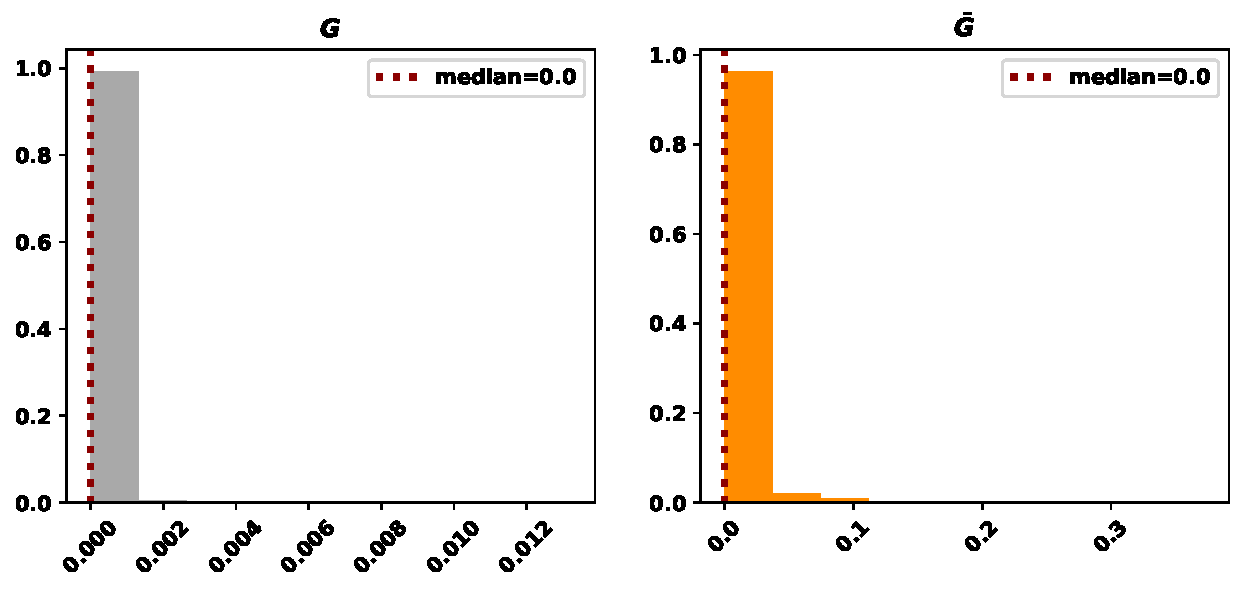
\includegraphics[width=.55\textwidth]{./assets/images/pd_betweeness_centralities.pdf}
    \caption{Distributions of betweenness centrality in \(G\) and \(\bar{G}\)}
    \label{fig:bc_distributions}
\end{figure}

\begin{figure}[!hbtp]
    \centering
    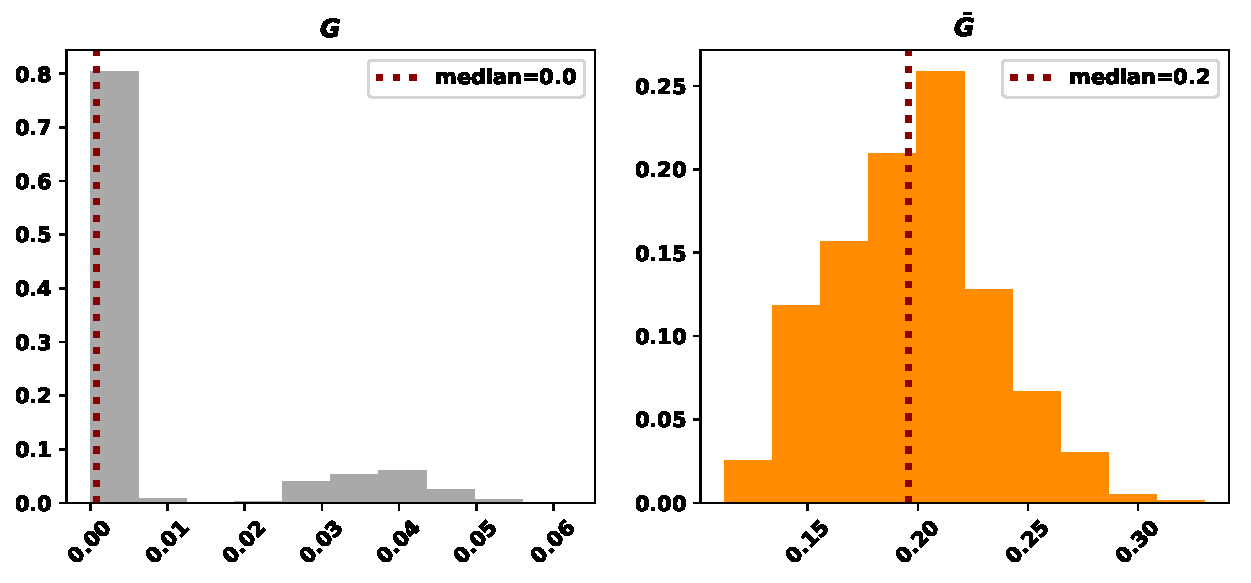
\includegraphics[width=.55\textwidth]{./assets/images/pd_closeness_centralities.pdf}
    \caption{Distributions of closeness centrality in \(G\) and \(\bar{G}\)}
    \label{fig:cc_distributions}
\end{figure}

\newcolumntype{g}{>{\columncolor{Gray}}l}
\begin{table}[!hbtp]
    \begin{center}
    \resizebox{.9\textwidth}{!}{\begin{tabular}{lggllggllgg}
\toprule
& \multicolumn{2}{g}{Topic A} & \multicolumn{2}{c}{Topic B} & \multicolumn{2}{g}{Topic C} & \multicolumn{2}{c}{Topic D} & \multicolumn{2}{g}{Topic E}\\
\midrule
{} &                 Name &  Betweeness &             Name &  Betweeness &             Name &  Betweeness &              Name &  Betweeness &                  Name &  Betweeness \\
\midrule
1  &           David Rand &       0.002 &        Long Wang &       0.006 &   Daniel Ashlock &       0.001 &       Matjaz Perc &       0.064 &             Zengru Di &         0.0 \\
2  &      Valerio Capraro &       0.001 &    Luo-Luo Jiang &       0.005 &      Matjaz Perc &       0.000 &     Luo-Luo Jiang &       0.037 &             Jian Yang &         0.0 \\
3  &        Angel Sanchez &       0.001 &     Martin Nowak &       0.004 &       Karl Tuyls &       0.000 &      Yamir Moreno &       0.031 &  Yevgeniy Vorobeychik &         0.0 \\
4  &              Feng Fu &       0.001 &      Matjaz Perc &       0.003 &  Philip Hingston &       0.000 &  Christoph Hauert &       0.027 &       Otavio Teixeira &         0.0 \\
5  &         Martin Nowak &       0.000 &  Attila Szolnoki &       0.003 &     Eun-Youn Kim &       0.000 &         Long Wang &       0.024 &      Roberto Oliveira &         0.0 \\
6  &  Nicholas Christakis &       0.000 &  Christian Hilbe &       0.002 &    Wendy Ashlock &       0.000 &         Zhen Wang &       0.024 &              M. Nowak &         0.0 \\
7  &   Pablo Branas-Garza &       0.000 &     Yamir Moreno &       0.002 &  Attila Szolnoki &       0.000 &      Han-Xin Yang &       0.023 &             M. Harper &         0.0 \\
8  &     Toshio Yamagishi &       0.000 &     Xiaojie Chen &       0.002 &       Seung Baek &       0.000 &      Martin Nowak &       0.020 &              Xiao Han &         0.0 \\
9  &         James Fowler &       0.000 &    Arne Traulsen &       0.002 &     Martin Nowak &       0.000 &     Angel Sanchez &       0.017 &            Zhesi Shen &         0.0 \\
10 &            Long Wang &       0.000 &        Zhen Wang &       0.002 &    Thore Graepel &       0.000 &       Zhihai Rong &       0.016 &           Wen-Xu Wang &         0.0 \\
\bottomrule
\end{tabular}
}
\end{center}
\caption{10 most central authors based on betweenness centrality
for topics' networks.}\label{table:central_authors_bc_topics}
\end{table}

\newcolumntype{g}{>{\columncolor{Gray}}l}
\begin{table}[!hbtp]
    \begin{center}
    \resizebox{.9\textwidth}{!}{\begin{tabular}{lggllggllgg}
\toprule
& \multicolumn{2}{g}{Topic A} & \multicolumn{2}{c}{Topic B} & \multicolumn{2}{g}{Topic C} & \multicolumn{2}{c}{Topic D} & \multicolumn{2}{g}{Topic E}\\
\midrule
{} &                 Name &  Closeness &               Name &  Closeness &                 Name &  Closeness &             Name &  Closeness &             Name &  Closeness \\
\midrule
1  &           David Rand &      0.027 &          Long Wang &      0.043 &           Karl Tuyls &      0.022 &      Matjaz Perc &      0.123 &  Stefanie Widder &      0.029 \\
2  &      Valerio Capraro &      0.023 &        Matjaz Perc &      0.041 &        Thore Graepel &      0.019 &        Zhen Wang &      0.109 &   Rosalind Allen &      0.029 \\
3  &       Jillian Jordan &      0.022 &    Attila Szolnoki &      0.040 &           Joel Leibo &      0.018 &        Long Wang &      0.107 &  Thomas Pfeiffer &      0.029 \\
4  &  Nicholas Christakis &      0.021 &       Martin Nowak &      0.040 &        Edward Hughes &      0.017 &     Yamir Moreno &      0.105 &    Thomas Curtis &      0.029 \\
5  &         James Fowler &      0.020 &  Olivier Tenaillon &      0.038 &     Matthew Phillips &      0.017 &    Luo-Luo Jiang &      0.104 &     Carsten Wiuf &      0.029 \\
6  &         Martin Nowak &      0.020 &       Xiaojie Chen &      0.038 &  Edgar Duenez-Guzman &      0.017 &  Attila Szolnoki &      0.103 &    William Sloan &      0.029 \\
7  &        Angel Sanchez &      0.019 &             Bin Wu &      0.038 &    Antonio Castaneda &      0.017 &     Gyorgy Szabo &      0.102 &     Otto Cordero &      0.029 \\
8  &    Gordon Kraft-Todd &      0.019 &      Yanling Zhang &      0.037 &         Iain Dunning &      0.017 &     Xiaojie Chen &      0.102 &        Sam Brown &      0.029 \\
9  &        Akihiro Nishi &      0.019 &            Feng Fu &      0.037 &             Tina Zhu &      0.017 &    Guangming Xie &      0.101 &     Babak Momeni &      0.029 \\
10 &        Anthony Evans &      0.019 &         David Rand &      0.037 &          Kevin Mckee &      0.017 &     Lucas Wardil &      0.101 &     Wenying Shou &      0.029 \\
\bottomrule
\end{tabular}
}
\end{center}
\caption{10 most central authors based on closeness centrality
for topics' networks.}\label{table:central_authors_cc_topics}
\end{table}

% \begin{figure}[!hbtp]
%     \centering
%     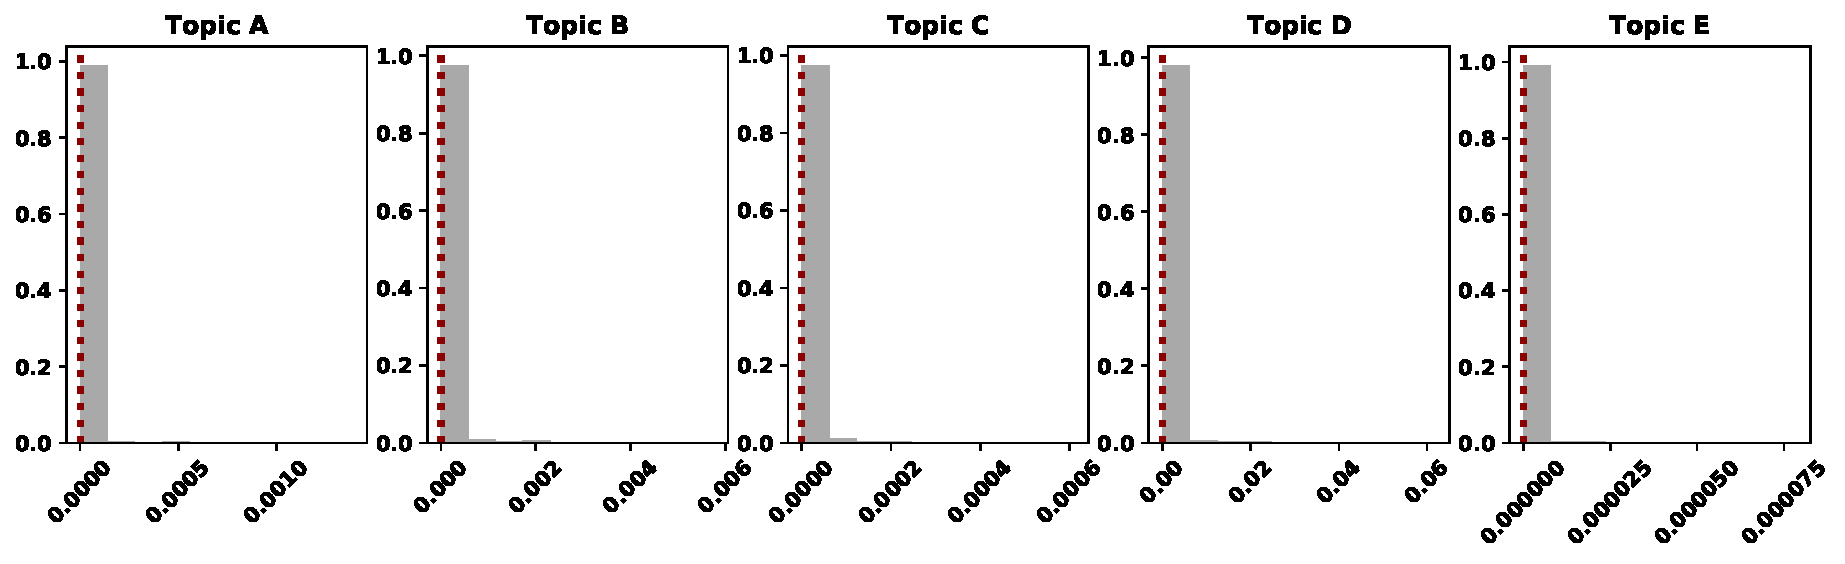
\includegraphics[width=.5\textwidth]{./assets/images/topics_betweeness_distributions.pdf}
%     \caption{Distributions of betweenness centrality in topics' networks.}
%     \label{fig:bc_distributions_topics}
% \end{figure}

% \begin{figure}[!hbtp]
%     \centering
%     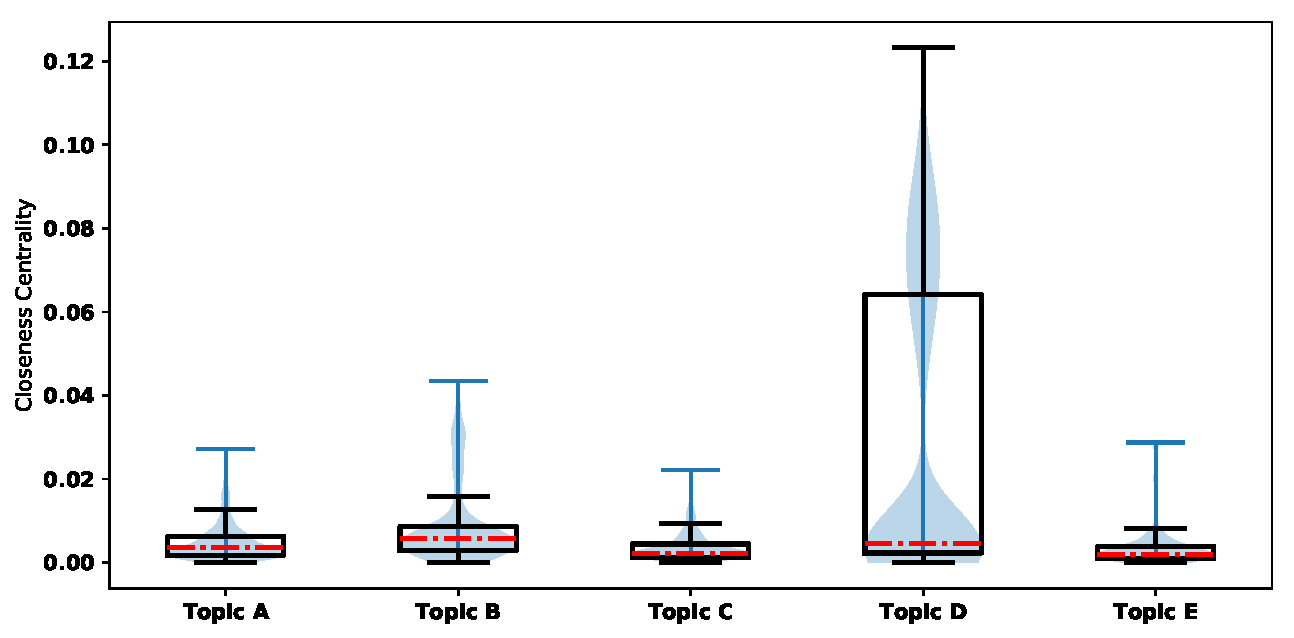
\includegraphics[width=.5\textwidth]{./assets/images/topics_closeness_distributions.pdf}
%     \caption{Distributions of closeness centrality in topics' networks.}
%     \label{fig:cc_distributions_topics}
% \end{figure}

\section{Conclusion}

This manuscript has explored the number of publications, the authors'
collaborative behaviour and their influence in the research topic of the Iterated
Prisoner's Dilemma. This was achieved by applying network theoretic approaches and
a bibliometric analysis in a data containing more than 2000 publications.
The data set was automatically
collected from five different sources using a bespoke piece of software written
for this purpose~\cite{nikoleta_2017}.

The data collection and an introduction to the methodology used in this work
were covered in Section~\ref{section:methodology}.
The data set contains a total of \totalarticles articles, it has been archive
and it available in~\cite{pd_data_2018} for further analysis.
Section~\ref{section:results} covered an initial analysis of the data set,
and applied a topic modeling algorithm which classified the articles into
topics. The initial analysis demonstrated that the field of the Prisoner's
Dilemma remains a prominent field with several papers being published in journals.
The topic modeling analysis identified five different topics which appeared
to be human subject research, biological studies, strategies and agent based simulations,
evolutionary dynamics on networks and modeling problems as a PD.
A temporal topic modeling analysis showed that over time not only
the number of topic changed, but also the scientific language and the most important
the topics authors were publishing on.

Following Section~\ref{section:results}, the collaborative behaviour of the field was explored
in Section~\ref{section:co_authorship}. It was concluded that the field
of the Iterated Prisoner's Dilemma is a collaborative field where authors
are likely to write with a collaborator's co-authors and on average an author
has 4 co-authors. The results on collaborativeness were verified when studying
the co-authorship network for each of the five topics defined in Section~\ref{section:results}
as well. Exploring the influence of authors and their gain from being in the
network of the field demonstrated that authors do not gain much, and the authors
with influence are the ones connected to the main cluster, to a "main" group of authors.

The study of the Prisoner's Dilemma is the study of cooperation and investigating
the cooperative behaviours of authors is what this work has aimed to achieve.
Interesting areas of future work would include extending this analysis to more
game theoretic sub fields, to evaluate whether the results remain the same.

\section{Acknowledgements}

A variety of software have been used in this work:

\begin{itemize}
    \item The Axelrod library for IPD simulations~\cite{axelrodproject}.
    \item The Matplotlib library for visualisation~\cite{hunter2007matplotlib}.
    \item The Numpy library for data manipulation~\cite{walt2011numpy}.
    \item The Networkx~\cite{networkx} package for analysing networks.
    \item Gephi~\cite{ICWSM09154} open source package for visualising networks.
    \item The Gensim library for the topic modeling~\cite{rehurek_lrec}.
    \item The louvain library for calculating the networks modularity \url{https://github.com/taynaud/python-louvain/issues}.
\end{itemize}

\bibliographystyle{plain}
\bibliography{bibliography.bib}
\end{document}